\textbf{CODE TABLE USED IN SECTION 0}

\textbf{Code table 0.0 -- \emph{Discipline of processed data in the GRIB message, number of GRIB Master\\
table}}

Code figure Meaning

0 Meteorological products

1 Hydrological products

2 Land surface products

3 Space products

4--9 Reserved

10 Oceanographic products

11--191 Reserved

192--254 Reserved for local use

255 Missing

\_\_\_\_\_\_\_\_\_\_\_\_

\textbf{CODE TABLES USED IN SECTION 1}

\textbf{Code table 1.0 -- \emph{GRIB master tables version number}}

Code figure Meaning

0 Experimental

1 Version implemented on 7 November 2001

2 Version implemented on 4 November 2003

3 Version implemented on 2 November 2005

4 Version implemented on 7 November 2007

5 Version implemented on 4 November 2009

6 Version implemented on 15 September 2010

7 Version implemented on 4 May 2011

8 Version implemented on 2 November 2011

9 Version implemented on 2 May 2012

10 Version implemented on 7 November 2012

11 Version implemented on 8 May 2013

12 Version implemented on 14 November 2013

13 Version implemented on 7 May 2014

14 Version implemented on 5 November 2014

15 Version implemented on 6 May 2015

16 Version implemented on 11 November 2015

17 Version implemented on 4 May 2016

18 Version implemented on 2 November 2016

19 Version implemented on 3 May 2017

20 Version implemented on 8 November 2017

21 Version implemented on 2 May 2018

22 Version implemented on 7 November 2018

23 Pre-operational to be implemented by next amendment

24--254 Future versions

255 Missing

Note: This code table is deprecated. See Common Code table C--0 instead.

\textbf{Code table 1.1 -- \emph{GRIB local tables version number}}

Code figure Meaning

0 Local tables not used. Only table entries and templates from the current master table\\
are valid

1--254 Number of local tables version used

255 Missing

\textbf{\\
}

\textbf{Code table 1.2 -- \emph{Significance of reference time}}

Code figure Meaning

0 Analysis

1 Start of forecast

2 Verifying time of forecast

3 Observation time

4--191 Reserved

192--254 Reserved for local use

255 Missing

\textbf{Code table 1.3 -- \emph{Production status of data}}

Code figure Meaning

0 Operational products

1 Operational test products

2 Research products

3 Re-analysis products

4 THORPEX Interactive Grand Global Ensemble (TIGGE)

5 THORPEX Interactive Grand Global Ensemble (TIGGE) test

6 S2S operational products

7 S2S test products

8 Uncertainties in Ensembles of Regional ReAnalyses project (UERRA)

9 Uncertainties in Ensembles of Regional ReAnalyses project (UERRA) test

10--191 Reserved

192--254 Reserved for local use

255 Missing

\textbf{Code table 1.4 -- \emph{Type of data}}

Code figure Meaning

0 Analysis products

1 Forecast products

2 Analysis and forecast products

3 Control forecast products

4 Perturbed forecast products

5 Control and perturbed forecast products

6 Processed satellite observations

7 Processed radar observations

8 Event probability

9--191 Reserved

192--254 Reserved for local use

255 Missing

Note: An initialized analysis is considered a zero-hour forecast.

\textbf{\\
}

\textbf{Code table 1.5 -- \emph{Identification template number}}

Code figure Meaning

0 Calendar definition

1 Paleontological offset

2 Calendar definition and paleontological offset

3--32767 Reserved

32768--65534 Reserved for local use

65535 Missing

\textbf{Code table 1.6 -- \emph{Type of calendar}}

Code figure Meaning Comments

0 Gregorian

1 360-day

2 365-day Essentially a non-leap year

3 Proleptic Gregorian Extends the Gregorian calendar indefinitely in the past

4--191 Reserved

192--254 Reserved for local use

255 Missing

\_\_\_\_\_\_\_\_\_\_\_\_\_\_

\textbf{CODE AND FLAG TABLES USED IN SECTION 3}

\textbf{Code table 3.0 -- \emph{Source of grid definition}}

Code figure Meaning Comments

0 Specified in Code table 3.1

1 Predetermined grid definition Defined by originating centre

2--191 Reserved

192--254 Reserved for local use

255 A grid definition does not apply to this product

\textbf{Code table 3.1 -- \emph{Grid definition template number}}

Code figure Meaning Comments

0 Latitude/longitude Also called equidistant cylindrical, or\\
Plate Carrée

1 Rotated latitude/longitude

2 Stretched latitude/longitude

3 Stretched and rotated latitude/longitude

4 Variable resolution latitude/longitude

5 Variable resolution rotated latitude/longitude

6--9 Reserved

10 Mercator

11--19 Reserved

20 Polar stereographic projection Can be south or north

21--29 Reserved

30 Lambert conformal Can be secant or tangent, conical or bipolar

31 Albers equal area

32--39 Reserved

40 Gaussian latitude/longitude

41 Rotated Gaussian latitude/longitude

42 Stretched Gaussian latitude/longitude

43 Stretched and rotated Gaussian latitude/longitude

44--49 Reserved

50 Spherical harmonic coefficients

51 Rotated spherical harmonic coefficients

52 Stretched spherical harmonic coefficients

53 Stretched and rotated spherical harmonic coefficients

54--89 Reserved

90 Space view perspective or orthographic

91--99 Reserved

100 Triangular grid based on an icosahedron

101 General unstructured grid

102--109 Reserved

110 Equatorial azimuthal equidistant projection

111--119 Reserved

120 Azimuth-range projection

121--139 Reserved

140 Lambert azimuthal equal area projection

141--999 Reserved

\emph{(continued)}

\emph{\\
(Code table 3.1 -- continued)}

Code figure Meaning

1000 Cross-section grid with points equally spaced on the horizontal

1001--1099 Reserved

1100 Hovmöller diagram grid with points equally spaced on the horizontal

1101--1199 Reserved

1200 Time section grid

1201--32767 Reserved

32768--65534 Reserved for local use

65535 Missing

\textbf{Code table 3.2 -- \emph{Shape of the Earth}}

Code figure Meaning

0 Earth assumed spherical with radius = 6 367 470.0 m

1 Earth assumed spherical with radius specified (in m) by data producer

2 Earth assumed oblate spheroid with size as determined by IAU in 1965 (major axis =\\
6 378 160.0 m, minor axis = 6 356 775.0 m, f = 1/297.0)

3 Earth assumed oblate spheroid with major and minor axes specified (in km) by data producer

4 Earth assumed oblate spheroid as defined in IAG-GRS80 model (major axis = 6 378 137.0 m, minor axis = 6 356 752.314 m, f = 1/298.257 222 101)

5 Earth assumed represented by WGS-84 (as used by ICAO since 1998)

6 Earth assumed spherical with radius of 6 371 229.0 m

7 Earth assumed oblate spheroid with major or minor axes specified (in m) by data producer

8 Earth model assumed spherical with radius of 6 371 200 m, but the horizontal datum of the resulting latitude/longitude field is the WGS-84 reference frame

9 Earth represented by the Ordnance Survey Great Britain 1936 Datum, using the Airy 1830 Spheroid, the Greenwich meridian as 0 longitude, and the Newlyn datum as mean sea level, 0~height

10--191 Reserved

192--254 Reserved for local use

255 Missing

Notes:

(1) WGS-84 is a geodetic system that uses IAG-GRS80 as a basis.

(2) With respect to code figures 0, 1, 3, 6 and 7, coordinates can only be unambiguously interpreted, if the coordinate reference system in which they are embedded is known. Therefore, defining the shape of the Earth alone without coordinate system axis origins is ambiguous. Generally, the prime meridian defined in the geodetic system WGS-84 can be safely assumed to be the longitudinal origin. However, because these code figures do not specify the longitudinal origin explicitly, it is suggested to contact the originating centre if high precision coordinates are needed, in order to obtain the precise details of the coordinate system used (effective as from 16 November 2016).

\textbf{Flag table 3.3 -- \emph{Resolution and component flags}}

Bit No. Value Meaning

1--2 Reserved

3 0 i direction increments not given

1 i direction increments given

4 0 j direction increments not given

1 j direction increments given

\emph{(continued)}

\emph{\\
(Flag table 3.3 -- continued)}

Bit No. Value Meaning

5 0 Resolved u- and v- components of vector quantities relative to easterly and northerly directions

1 Resolved u- and v- components of vector quantities relative to the defined grid in the direction of increasing x and y (or i and j) coordinates, respectively

6--8 Reserved -- set to zero

\textbf{Flag table 3.4 -- \emph{Scanning mode}}

Bit No. Value Meaning

1 0 Points of first row or column scan in the +i (+x) direction

1 Points of first row or column scan in the --i (--x) direction

2 0 Points of first row or column scan in the --j (--y) direction

1 Points of first row or column scan in the +j (+y) direction

3 0 Adjacent points in i (x) direction are consecutive

1 Adjacent points in j (y) direction is consecutive

4 0 All rows scan in the same direction

1 Adjacent rows scans in the opposite direction

5 0 Points within odd rows are not offset in i (x) direction

1 Points within odd rows are offset by Di/2 in i (x) direction

6 0 Points within even rows are not offset in i (x) direction

1 Points within even rows are offset by Di/2 in i (x) direction

7 0 Points are not offset in j (y) direction

1 Points are offset by Dj/2 in j (y) direction

8 0 Rows have Ni grid points and columns have Nj grid points

1 Rows have Ni grid points if points are not offset in i direction

Rows have Ni--1 grid points if points are offset by Di/2 in i direction

Columns have Nj grid points if points are not offset in j direction

Columns have Nj--1 grid points if points are offset by Dj/2 in j direction

Notes:

(1) i direction: west to east along a parallel or left to right along an x-axis.

(2) j direction: south to north along a meridian, or bottom to top along a y-axis.

(3) If bit number 4 is set, the first row scan is as defined by previous flags.

(4) La1 and Lo1 define the first row, which is an odd row.

(5) Di and Dj are assumed to be positive, with the direction of i and j being given by bits 1 and 2.

(6) Bits 5 through 8 may be used to generate staggered grids, such as Arakawa grids (see Part B, GRIB Attachment II).

(7) If any of bits 5, 6, 7 or 8 are set, Di and Dj are not optional.

\textbf{Flag table 3.5 -- \emph{Projection }}\emph{centre}

Bit No. Value Meaning

1 0 North Pole is on the projection plane

1 South Pole is on the projection plane

2 0 Only one projection centre is used

1 Projection is bipolar and symmetric

\textbf{\\
}

\textbf{Code table 3.6 -- \emph{Spectral data representation type}}

Code figure Meaning

1 The associated Legendre functions of the first kind are defined by:

\begin{quote}
= 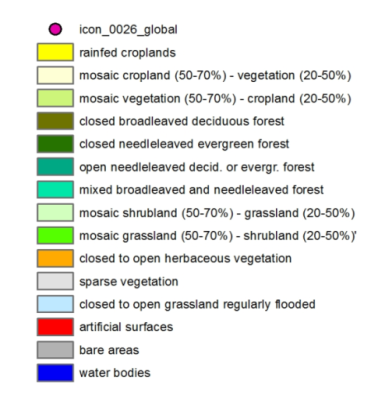
\includegraphics{../tex/extracted-media/media/image2.wmf}

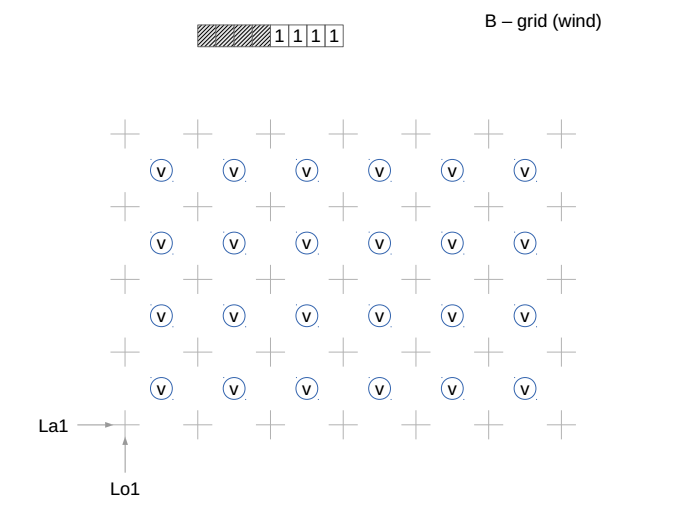
\includegraphics{../tex/extracted-media/media/image3.wmf}
\end{quote}

A field \emph{F(λ,} μ) is represented by:

\begin{quote}
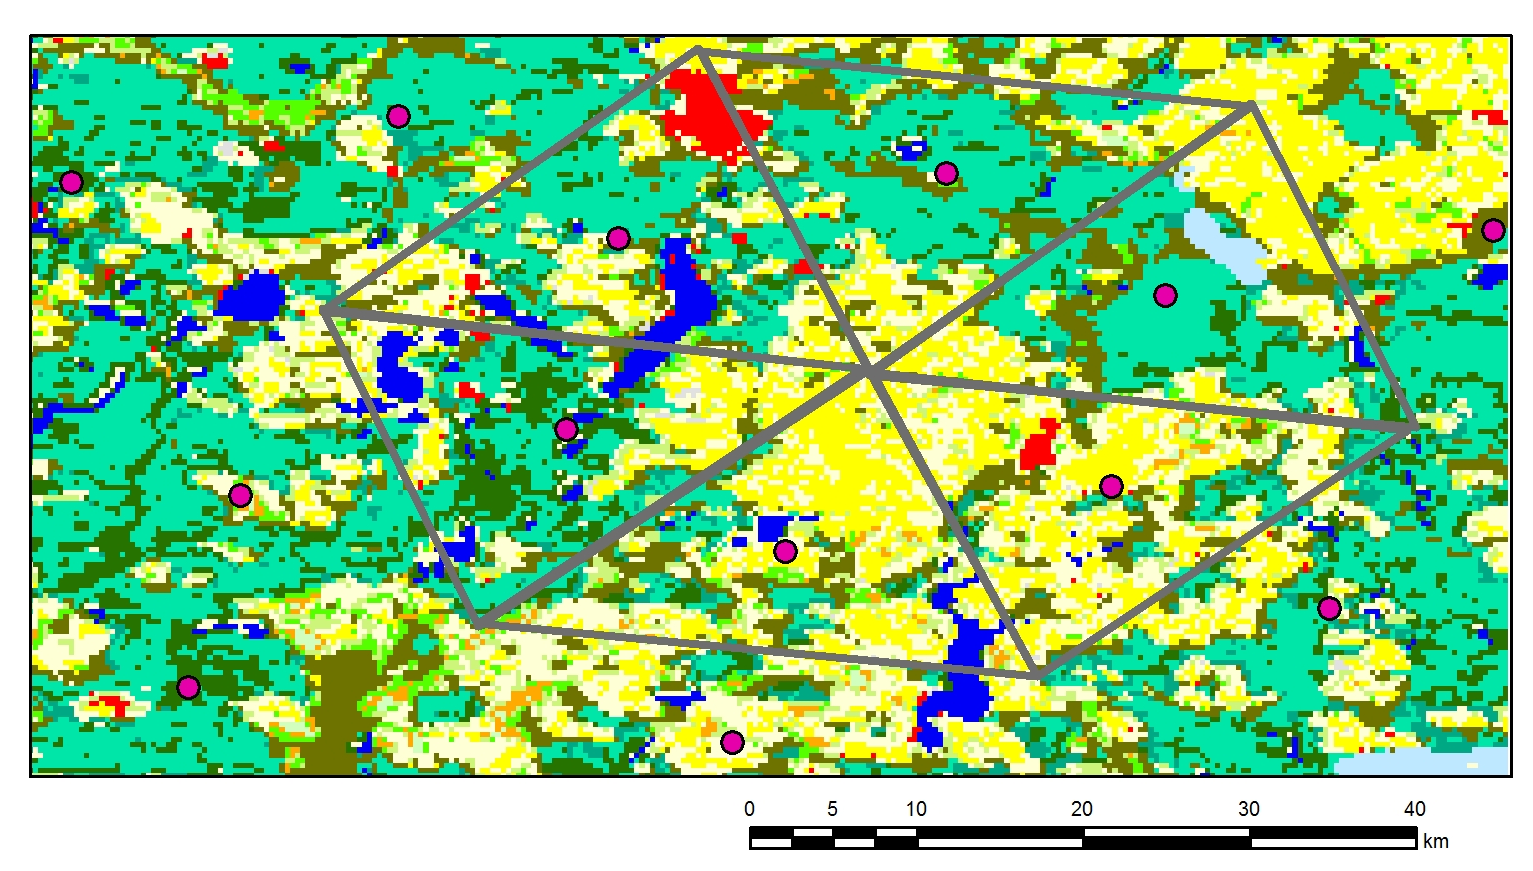
\includegraphics{../tex/extracted-media/media/image4.wmf}
\end{quote}

where 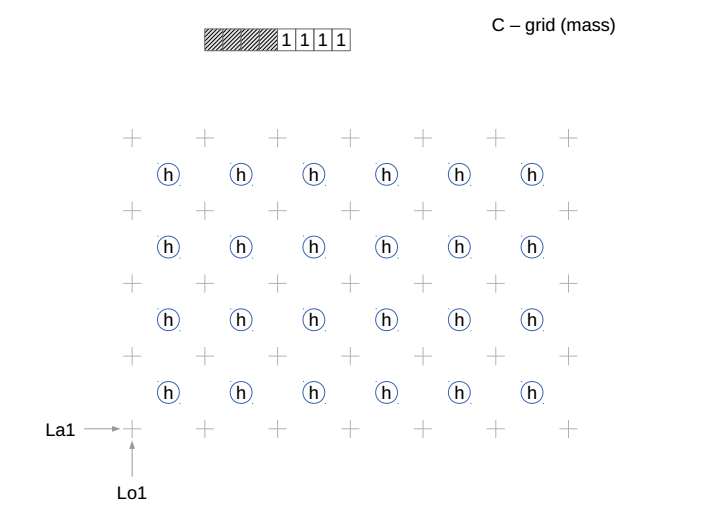
\includegraphics{../tex/extracted-media/media/image5.wmf}is the longitude,

\begin{quote}
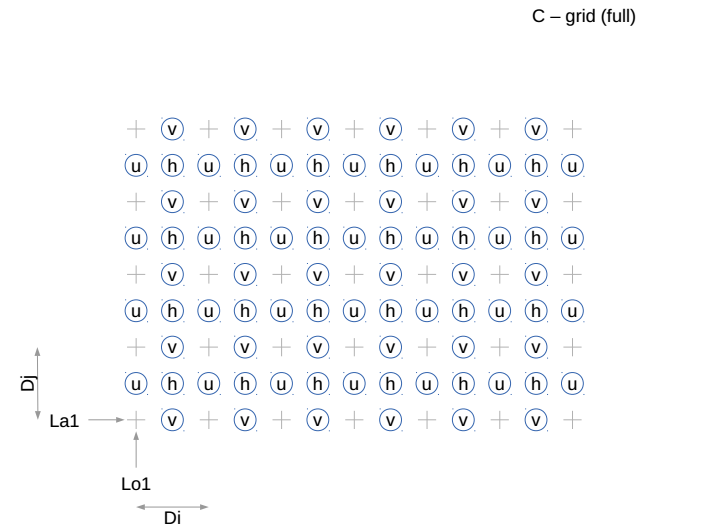
\includegraphics{../tex/extracted-media/media/image6.wmf} the sine of latitude,

and 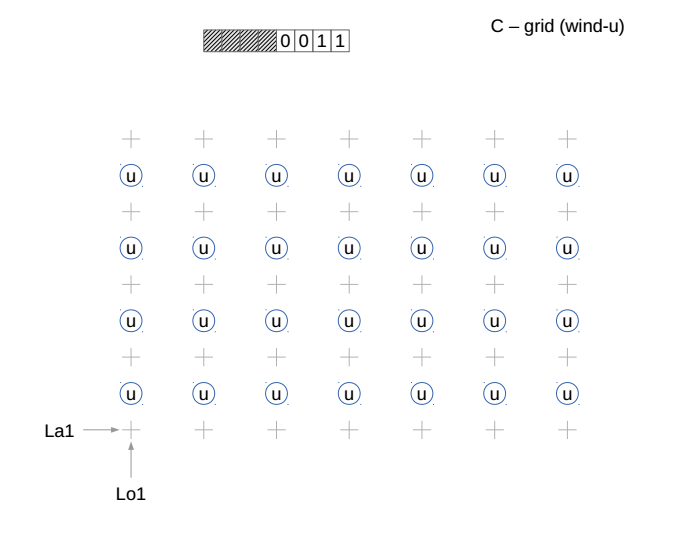
\includegraphics{../tex/extracted-media/media/image7.wmf} the complex conjugate of 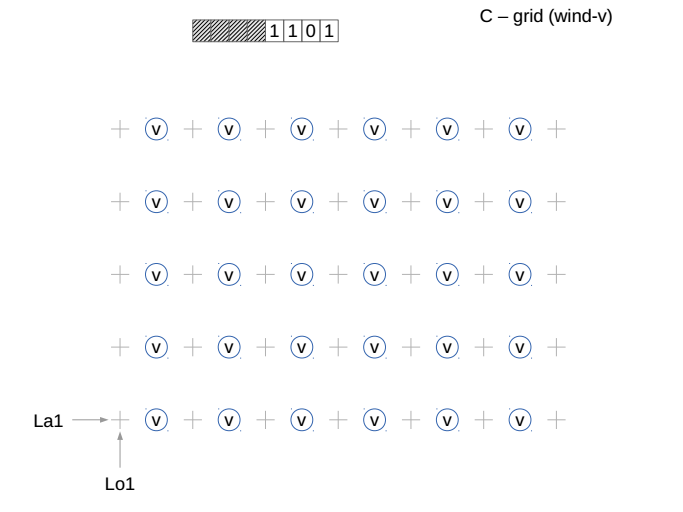
\includegraphics{../tex/extracted-media/media/image8.wmf}
\end{quote}

\textbf{Code table 3.7 -- \emph{Spectral data representation mode}}

Code figure Meaning

0 Reserved

1 The complex numbers 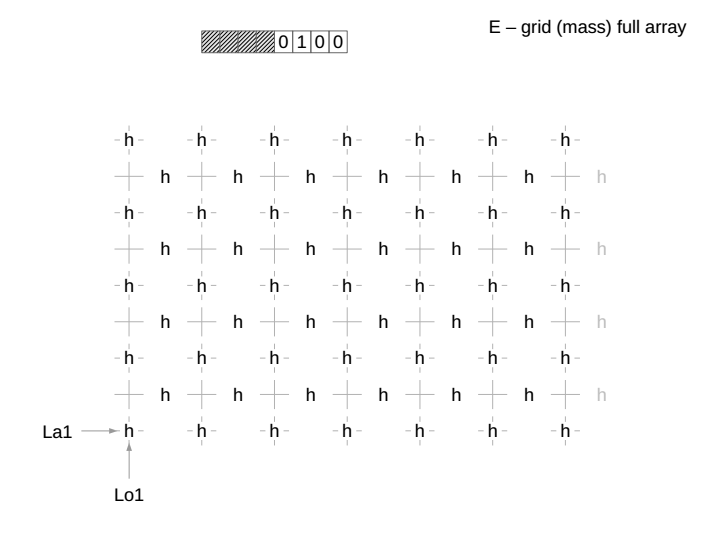
\includegraphics[width=0.21319in,height=0.23333in]{../tex/extracted-media/media/image9.wmf}(see code figure 1 in Code table 3.6) are stored for m ≥ 0 as\\
pairs of real numbers Re(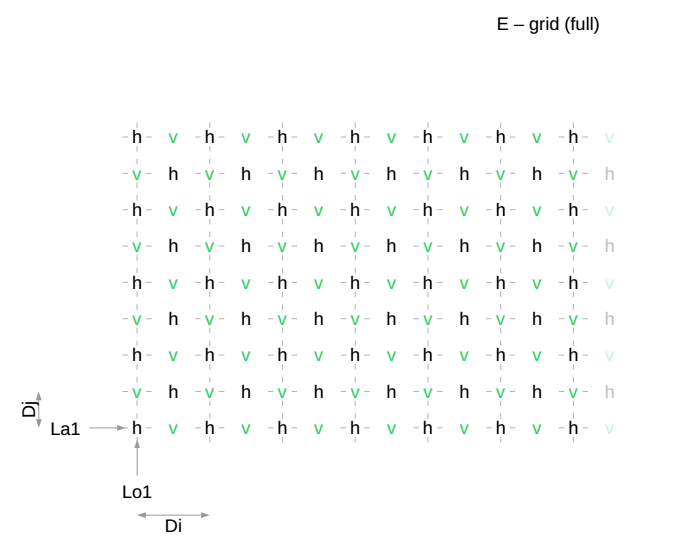
\includegraphics[width=0.21319in,height=0.23333in]{../tex/extracted-media/media/image10.wmf}), Im(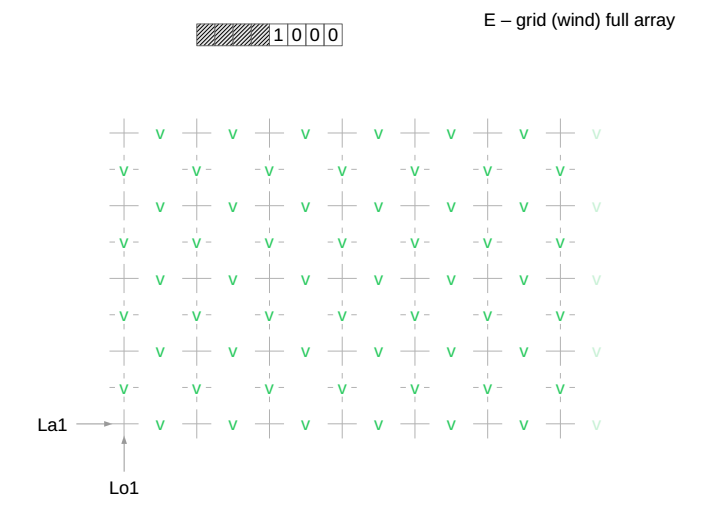
\includegraphics[width=0.21319in,height=0.23333in]{../tex/extracted-media/media/image11.wmf}) ordered with n increasing from m to N(m), first for\\
m = 0 and then for m = 1, 2, ... M (see Note)

2--254 Reserved

255 Missing

Note: Values of N(m) for common truncation cases:

Triangular: M = J = K, N(m) = J

Rhomboidal: K = J + M, N(m) = J + m

Trapezoidal: K = J, K \textgreater{} M, N(m) = J

\textbf{Code table 3.8 -- \emph{Grid point position}}

Code figure Meaning

0 Grid points at triangle vertices

1 Grid points at centres of triangles

2 Grid points at midpoints of triangle sides

3--191 Reserved

192--254 Reserved for local use

255 Missing

\textbf{Flag table 3.9 -- \emph{Numbering order of diamonds as seen from the corresponding pole}}

Bit No. Value Meaning

1 0 Clockwise orientation

1 Anti-clockwise (i.e. counter-clockwise) orientation

2--8 Reserved

\textbf{\\
}

\textbf{Flag table 3.10 -- \emph{Scanning mode for one diamond}}

Bit No. Value Meaning

1 0 Points scan in +i direction, i.e. from pole to Equator

1 Points scan in --i direction, i.e. from Equator to pole

2 0 Points scan in +j direction, i.e. from west to east

1 Points scan in --j direction, i.e. from east to west

3 0 Adjacent points in i direction are consecutive

1 Adjacent points in j direction are consecutive

4--8 Reserved

\textbf{Code table 3.11 -- \emph{Interpretation of list of numbers at end of section 3}}

Code figure Meaning

0 There is no appended list

1 Numbers define number of points corresponding to full coordinate circles (i.e. parallels),\\
coordinate values on each circle are multiple of the circle mesh, and extreme coordinate\\
values given in grid definition (i.e. extreme longitudes) may not be reached in all rows

2 Numbers define number of points corresponding to coordinate lines delimited by extreme\\
coordinate values given in grid definition (i.e. extreme longitudes) which are present in\\
each row

3 Numbers define the actual latitudes for each row in the grid. The list of numbers are integer\\
values of the valid latitudes in microdegrees (scaled by 10\textsuperscript{--6}) or in unit equal to the ratio of\\
the basic angle and the subdivisions number for each row, in the same order as specified\\
in the "scanning mode flag" (bit no. 2) (see Note 2)

4--254 Reserved

255 Missing

Notes:

(1) For entry 1, it should be noted that depending on values of extreme (first/last) coordinates, and regardless of bit-map, effective number of points per row may be less than the number of points on the current circle.

(2) The value for the constant direction increment Di (or Dx) in the accompanying grid definition template should be set to all ones (missing).

\textbf{Code table 3.15 -- \emph{Physical meaning of vertical coordinate}}

Code figure Meaning Unit

0--19 Reserved

20 Temperature K

21--99 Reserved

100 Pressure Pa

101 Pressure deviation from mean sea level Pa

102 Altitude above mean sea level m

103 Height above ground (see Note 1) m

104 Sigma coordinate

105 Hybrid coordinate

106 Depth below land surface m

107 Potential temperature (theta) K

108 Pressure deviation from ground to level Pa

109 Potential vorticity K m\textsuperscript{--2} kg\textsuperscript{--1} s\textsuperscript{--1}

110 Geometrical height m

\emph{(continued)}

\emph{\\
(Code table 3.15 -- continued)}

Code figure Meaning Unit

111 Eta coordinate (see Note 2)

112 Geopotential height gpm

113 Logarithmic hybrid coordinate

114--159 Reserved

160 Depth below sea level m

161--191 Reserved

192--254 Reserved for local use

255 Missing

Notes:

(1) Negative values associated to this coordinate will indicate depth below ground surface. If values are all below surface, use of entry 10\textsuperscript{6} is recommended, with positive coordinate values instead.

(2) The Eta vertical coordinate system involves normalizing the pressure at some point on a specific level by the mean sea-level pressure at that point.

\textbf{Code table 3.20 -- \emph{Type of horizontal line}}

Code figure Meaning

0 Rhumb

1 Great circle

2--191 Reserved

192--254 Reserved for local use

255 Missing

\textbf{Code table 3.21 \emph{-- Vertical dimension coordinate values definition}}

Code figure Meaning

0 Explicit coordinate values set

1 Linear coordinates\\
f(1) = C1\\
f(n) = f(n--1) + C2

2--10 Reserved

11 Geometric coordinates\\
f(1) = C1\\
f(n) = C2 × f(n--1)

12--191 Reserved

192--254 Reserved for local use

255 Missing

\_\_\_\_\_\_\_\_\_\_\_\_

\textbf{CODE TABLES USED IN SECTION 4}

\textbf{Code table 4.0 -- \emph{Product definition template number}}

Code figure Meaning

0 Analysis or forecast at a horizontal level or in a horizontal layer at a point in time

1 Individual ensemble forecast, control and perturbed, at a horizontal level or in a\\
horizontal layer at a point in time

2 Derived forecasts based on all ensemble members at a horizontal level or in a\\
horizontal layer at a point in time

3 Derived forecasts based on a cluster of ensemble members over a rectangular area at a\\
horizontal level or in a horizontal layer at a point in time

4 Derived forecasts based on a cluster of ensemble members over a circular area at a\\
horizontal level or in a horizontal layer at a point in time

5 Probability forecasts at a horizontal level or in a horizontal layer at a point in time

6 Percentile forecasts at a horizontal level or in a horizontal layer at a point in time

7 Analysis or forecast error at a horizontal level or in a horizontal layer at a point in time

8 Average, accumulation, extreme values or other statistically processed values at a\\
horizontal level or in a horizontal layer in a continuous or non-continuous time interval

9 Probability forecasts at a horizontal level or in a horizontal layer in a continuous or\\
non-continuous time interval

10 Percentile forecasts at a horizontal level or in a horizontal layer in a continuous or non-\\
continuous time interval

11 Individual ensemble forecast, control and perturbed, at a horizontal level or in a\\
horizontal layer, in a continuous or non-continuous interval

12 Derived forecasts based on all ensemble members at a horizontal level or in a horizontal\\
layer, in a continuous or non-continuous interval

13 Derived forecasts based on a cluster of ensemble members over a rectangular area, at\\
a horizontal level or in a horizontal layer, in a continuous or non-continuous interval

14 Derived forecasts based on a cluster of ensemble members over a circular area, at a\\
horizontal level or in a horizontal layer, in a continuous or non-continuous interval

15 Average, accumulation, extreme values, or other statistically processed values over a\\
spatial area at a horizontal level or in a horizontal layer at a point in time

16--19 Reserved

20 Radar product

21--29 Reserved

30 Satellite product (deprecated)

31 Satellite product

32 Analysis or forecast at a horizontal level or in a horizontal layer at a point in time for\\
simulated (synthetic) satellite data

33 Individual ensemble forecast, control and perturbed, at a horizontal level or in a horizontal\\
layer at a point in time for simulated (synthetic) satellite data

34 Individual ensemble forecast, control and perturbed, at a horizontal level or in a horizontal\\
layer, in a continuous or non-continuous interval for simulated (synthetic) satellite data

35--39 Reserved

40 Analysis or forecast at a horizontal level or in a horizontal layer at a point in time for\\
atmospheric chemical constituents

41 Individual ensemble forecast, control and perturbed, at a horizontal level or in a\\
horizontal layer at a point in time for atmospheric chemical constituents

42 Average, accumulation and/or extreme values or other statistically processed values at\\
a horizontal level or in a horizontal layer in a continuous or non-continuous time interval\\
for atmospheric chemical constituents

\emph{(continued)}

\emph{\\
(Code table 4.0 -- continued)}

Code figure Meaning

43 Individual ensemble forecast, control and perturbed, at a horizontal level or in a\\
horizontal layer in a continuous or non-continuous time interval for atmospheric\\
chemical constituents

44 Analysis or forecast at a horizontal level or in a horizontal layer at a point in time for\\
aerosol

45 Individual ensemble forecast, control and perturbed, at a horizontal level or in\\
a horizontal layer at a point in time for aerosol

46 Average, accumulation, and/or extreme values or other statistically processed values\\
at a horizontal level or in a horizontal layer in a continuous or non-continuous time\\
interval for aerosol

47 Individual ensemble forecast, control and perturbed, at a horizontal level or in\\
a horizontal layer in a continuous or non-continuous time interval for aerosol

48 Analysis or forecast at a horizontal level or in a horizontal layer at a point in time for\\
optical properties of aerosol

49 Individual ensemble forecast, control and perturbed, at a horizontal level or in a horizontal\\
layer at a point in time for optical properties of aerosol

50 Reserved

51 Categorical forecasts at a horizontal level or in a horizontal layer at a point in time

52 Reserved

53 Partitioned parameters at a horizontal level or in a horizontal layer at a point in time

54 Individual ensemble forecast, control and perturbed, at a horizontal level or in a horizontal\\
layer at a point in time for partitioned parameters

55 Spatio-temporal changing tiles at a horizontal level or horizontal layer at a point in time

56 Individual ensemble forecast, control and perturbed, at a horizontal level or in a horizontal\\
layer at a point in time for spatio-temporal changing tile parameters (deprecated)

57 Analysis or forecast at a horizontal level or in a horizontal layer at a point in time for\\
atmospheric chemical constituents based on a distribution function

58 Individual ensemble forecast, control and perturbed, at a horizontal level or in a horizontal\\
layer at a point in time for atmospheric chemical constituents based on a distribution\\
function

59 Individual ensemble forecast, control and perturbed, at a horizontal level or in a horizontal\\
layer at a point in time for spatio-temporal changing tile parameters (corrected version of\\
template 4.56)

60 Individual ensemble reforecast, control and perturbed, at a horizontal level or in a horizontal\\
layer at a point in time

61 Individual ensemble reforecast, control and perturbed, at a horizontal level or in a horizontal\\
layer, in a continuous or non-continuous time interval

62--66 Reserved

67 Average, accumulation and/or extreme values or other statistically processed values at\\
a horizontal level or in a horizontal layer in a continuous or non-continuous time interval for\\
atmospheric chemical constituents based on a distribution function

68 Individual ensemble forecast, control and perturbed, at a horizontal level or in a horizontal\\
layer in a continuous or non-continuous time interval for atmospheric chemical constituents\\
based on a distribution function

69 Reserved

70 Post-processing analysis or forecast at a horizontal level or in a horizontal layer at a point in time

71 Post-processing individual ensemble forecast, control and perturbed, at a horizontal level or in a\\
horizontal layer at a point in time

72 Post-processing average, accumulation, extreme values or other statistically processed values at a\\
horizontal level or in a horizontal layer in a continuous or non-continuous time interval

73 Post-processing individual ensemble forecast, control and perturbed, at a horizontal level or in a\\
horizontal layer, in a continuous or non-continuous time interval

\emph{(continued)}

\emph{\\
(Code table 4.0 -- continued)}

Code figure Meaning

74--90 Reserved

91 Categorical forecasts at a horizontal level or in a horizontal layer in a continuous or\\
non-continuous time interval

92--253 Reserved

254 CCITT IA5 character string

255--999 Reserved

1000 Cross-section of analysis and forecast at a point in time

1001 Cross-section of averaged or otherwise statistically processed analysis or forecast over a\\
range of time

1002 Cross-section of analysis and forecast, averaged or otherwise statistically processed over\\
latitude or longitude

1003--1099 Reserved

1100 Hovmöller-type grid with no averaging or other statistical processing

1101 Hovmöller-type grid with averaging or other statistical processing

1102--32767 Reserved

32768--65534 Reserved for local use

65535 Missing

\textbf{Code table 4.1 --} \emph{Parameter category by product discipline}

Note: When a new category is to be added to Code table 4.1 and more than one discipline applies, the choice of discipline should be made based on the intended use of the product.

\textbf{Product discipline 0 -- Meteorological products}

Category Description

0 Temperature

1 Moisture

2 Momentum

3 Mass

4 Short-wave radiation

5 Long-wave radiation

6 Cloud

7 Thermodynamic stability indices

8 Kinematic stability indices

9 Temperature probabilities

10 Moisture probabilities

11 Momentum probabilities

12 Mass probabilities

13 Aerosols

14 Trace gases (e.g. ozone, CO\textsubscript{2})

15 Radar

16 Forecast radar imagery

17 Electrodynamics

18 Nuclear/radiology

19 Physical atmospheric properties

20 Atmospheric chemical constituents

21--189 Reserved

\emph{(continued)}

\emph{\\
(Code table 4.1 -- continued)}

190 CCITT IA5 string

191 Miscellaneous

192--254 Reserved for local use

255 Missing

Note: Entries 9, 10, 11 and 12 are deprecated.

\textbf{Product discipline 1 -- Hydrological products}

Category Description

0 Hydrology basic products

1 Hydrology probabilities

2 Inland water and sediment properties

3--191 Reserved

192--254 Reserved for local use

255 Missing

\textbf{Product discipline 2 -- Land surface products}

Category Description

0 Vegetation/biomass

1 Agri-/aquacultural special products

2 Transportation-related products

3 Soil products

4 Fire weather products

5--191 Reserved

192--254 Reserved for local use

255 Missing

\textbf{Product discipline 3 -- Space products}

Category Description

0 Image format products (see Note 1)

1 Quantitative products (see Note 2)

2 Cloud properties

3 Flight rule conditions

4 Volcanic ash

5 Sea-surface temperature

6 Solar radiation

7--191 Reserved

192--254 Reserved for local use

255 Missing

Notes:

(1) Data are numeric without units, although they might be given quantitative meaning through a code table defined external to this document. The emphasis is on a displayable ``picture'' of some phenomenon, perhaps with certain enhanced features. Generally, each datum is an unsigned, one octet integer, but some image format products might have another datum size. The size of a datum is indicated in section 5.

(2) Data are in specified physical units.

\emph{(continued)}

\textbf{\\
}

\emph{(Code table 4.1 -- continued)}

\textbf{Product discipline 10 -- Oceanographic products}

Category Description

0 Waves

1 Currents

2 Ice

3 Surface properties

4 Subsurface properties

5--190 Reserved

191 Miscellaneous

192--254 Reserved for local use

255 Missing

\textbf{Code table 4.2} \textbf{--} \emph{Parameter number by product discipline and parameter category}

Notes:

(1) By convention, the flux sign is positive if downwards.

(2) When a new parameter is to be added to Code table 4.2 and more than one category applies, the choice of category should be made based on the intended use of the product. The discipline and category are an important part of any product definition, so it is possible to have the same parameter name in more than one category. For example, ``water temperature'' in discipline 10 (oceanographic products), category 4 (subsurface properties) is used for reporting water temperature in the ocean or open sea, and is not the same as ``water temperature'' in discipline 1 (hydrological products), category 2 (inland water and sediment properties), which is used for reporting water temperature in freshwater lakes and rivers.

\textbf{Product discipline 0 -- Meteorological products, parameter category 0: temperature}

Number Parameter Units

0 Temperature K

1 Virtual temperature K

2 Potential temperature K

3 Pseudo-adiabatic potential temperature K\\
or equivalent potential temperature

4 Maximum temperature* K

5 Minimum temperature* K

6 Dewpoint temperature K

7 Dewpoint depression (or deficit) K

8 Lapse rate K m\textsuperscript{--1}

9 Temperature anomaly K

10 Latent heat net flux W m\textsuperscript{--2}

11 Sensible heat net flux W m\textsuperscript{--2}

12 Heat index K

13 Wind chill factor K

14 Minimum dewpoint depression* K

15 Virtual potential temperature K

16 Snow phase change heat flux W m\textsuperscript{--2}

17 Skin temperature K

18 Snow temperature (top of snow) K

19 Turbulent transfer coefficient for heat Numeric

20 Turbulent diffusion coefficient for heat m\textsuperscript{2} s\textsuperscript{--1}

\emph{(continued)}

\emph{\\
(Code table 4.2 -- continued)}

Number Parameter Units

21 Apparent temperature** K

22 Temperature tendency due to short-wave radiation K s\textsuperscript{--1}

23 Temperature tendency due to long-wave radiation K s\textsuperscript{--1}

24 Temperature tendency due to short-wave radiation, K s\textsuperscript{--1}\\
clear sky

25 Temperature tendency due to long-wave radiation, K s\textsuperscript{--1}\\
clear sky

26 Temperature tendency due to parameterization K s\textsuperscript{--1}

27 Wet-bulb temperature K

28 Unbalanced component of temperature K

29 Temperature advection K s\textsuperscript{\emph{\textbf{--}}1}

30--191 Reserved

192--254 Reserved for local use

255 Missing

\_\_\_\_\_\_\_\_\_\_\_\_\_\_\_\_\_\_\_\_\_

* Parameter deprecated. See Regulation 92.6.2 and use another parameter instead.

** Apparent temperature is the perceived outdoor temperature, caused by a combination of phenomena, such as air temperature, relative humidity and wind speed.

\textbf{Product discipline 0 -- Meteorological products, parameter category 1: moisture}

Number Parameter Units

0 Specific humidity kg kg\textsuperscript{--1}

1 Relative humidity \%

2 Humidity mixing ratio kg kg\textsuperscript{--1}

3 Precipitable water kg m\textsuperscript{--2}

4 Vapour pressure Pa

5 Saturation deficit Pa

6 Evaporation kg m\textsuperscript{--2}

7 Precipitation rate* kg m\textsuperscript{--2} s\textsuperscript{--1}

8 Total precipitation*** kg m\textsuperscript{--2}

9 Large-scale precipitation (non-convective)*** kg m\textsuperscript{--2}

10 Convective precipitation*** kg m\textsuperscript{--2}

11 Snow depth m

12 Snowfall rate water equivalent* kg m\textsuperscript{--2} s\textsuperscript{--1}

13 Water equivalent of accumulated snow depth*** kg m\textsuperscript{--2}

14 Convective snow*** kg m\textsuperscript{--2}

15 Large-scale snow*** kg m\textsuperscript{--2}

16 Snow melt kg m\textsuperscript{--2}

17 Snow age d

18 Absolute humidity kg m\textsuperscript{--3}

19 Precipitation type (Code table 4.201)

20 Integrated liquid water kg m\textsuperscript{--2}

21 Condensate kg kg\textsuperscript{--1}

22 Cloud mixing ratio kg kg\textsuperscript{--1}

23 Ice water mixing ratio kg kg\textsuperscript{--1}

24 Rain mixing ratio kg kg\textsuperscript{--1}

\emph{(continued)}

\emph{\\
(Code table 4.2 -- continued)}

Number Parameter Units

25 Snow mixing ratio kg kg\textsuperscript{--1}

26 Horizontal moisture convergence kg kg\textsuperscript{--1} s\textsuperscript{--1}

27 Maximum relative humidity* \%

28 Maximum absolute humidity* kg m\textsuperscript{--3}

29 Total snowfall*** m

30 Precipitable water category (Code table 4.202)

31 Hail m

32 Graupel (snow pellets) kg kg\textsuperscript{--1}

33 Categorical rain (Code table 4.222)

34 Categorical freezing rain (Code table 4.222)

35 Categorical ice pellets (Code table 4.222)

36 Categorical snow (Code table 4.222)

37 Convective precipitation rate kg m\textsuperscript{--2} s\textsuperscript{--1}

38 Horizontal moisture divergence kg kg\textsuperscript{--1} s\textsuperscript{--1}

39 Per cent frozen precipitation \%

40 Potential evaporation kg m\textsuperscript{--2}

41 Potential evaporation rate W m\textsuperscript{--2}

42 Snow cover \%

43 Rain fraction of total cloud water Proportion

44 Rime factor Numeric

45 Total column integrated rain kg m\textsuperscript{--2}

46 Total column integrated snow kg m\textsuperscript{--2}

47 Large scale water precipitation (non-convective)*** kg m\textsuperscript{--2}

48 Convective water precipitation*** kg m\textsuperscript{--2}

49 Total water precipitation*** kg m\textsuperscript{--2}

50 Total snow precipitation*** kg m\textsuperscript{--2}

51 Total column water (Vertically integrated total water kg m\textsuperscript{--2}\\
(vapour + cloud water/ice))

52 Total precipitation rate** kg m\textsuperscript{--2} s\textsuperscript{--1}

53 Total snowfall rate water equivalent** kg m\textsuperscript{--2} s\textsuperscript{--1}

54 Large scale precipitation rate kg m\textsuperscript{--2} s\textsuperscript{--1}

55 Convective snowfall rate water equivalent kg m\textsuperscript{--2} s\textsuperscript{--1}

56 Large scale snowfall rate water equivalent kg m\textsuperscript{--2} s\textsuperscript{--1}

57 Total snowfall rate m s\textsuperscript{--1}

58 Convective snowfall rate m s\textsuperscript{--1}

59 Large scale snowfall rate m s\textsuperscript{--1}

60 Snow depth water equivalent kg m\textsuperscript{--2}

61 Snow density kg m\textsuperscript{--3}

62 Snow evaporation kg m\textsuperscript{--2}

63 Reserved

64 Total column integrated water vapour kg m\textsuperscript{--2}

65 Rain precipitation rate kg m\textsuperscript{--2} s\textsuperscript{--1}

66 Snow precipitation rate kg m\textsuperscript{--2} s\textsuperscript{--1}

67 Freezing rain precipitation rate kg m\textsuperscript{--2} s\textsuperscript{--1}

68 Ice pellets precipitation rate kg m\textsuperscript{--2} s\textsuperscript{--1}

\emph{(continued)}

\emph{\\
(Code table 4.2 -- continued)}

Number Parameter Units

69 Total column integrated cloud water kg m\textsuperscript{--2}

70 Total column integrated cloud ice kg m\textsuperscript{--2}

71 Hail mixing ratio kg kg\textsuperscript{--1}

72 Total column integrated hail kg m\textsuperscript{--2}

73 Hail precipitation rate kg m\textsuperscript{--2} s\textsuperscript{--1}

74 Total column integrated graupel kg m\textsuperscript{--2}

75 Graupel (snow pellets) precipitation rate kg m\textsuperscript{--2} s\textsuperscript{--1}

76 Convective rain rate kg m\textsuperscript{--2} s\textsuperscript{--1}

77 Large scale rain rate kg m\textsuperscript{--2} s\textsuperscript{--1}

78 Total column integrated water (all components kg m\textsuperscript{--2}\\
including precipitation)

79 Evaporation rate kg m\textsuperscript{--2} s\textsuperscript{--1}

80 Total condensate kg kg\textsuperscript{--1}

81 Total column-integrated condensate kg m\textsuperscript{--2}

82 Cloud ice mixing-ratio kg kg\textsuperscript{--1}

83 Specific cloud liquid water content kg kg\textsuperscript{--1}

84 Specific cloud ice water content kg kg\textsuperscript{--1}

85 Specific rainwater content kg kg\textsuperscript{--1}

86 Specific snow water content kg kg\textsuperscript{--1}

87 \textbf{Stratiform precipitation rate kg m}\textsuperscript{--\textbf{2}} \textbf{s}\textsuperscript{--\textbf{1}}

88 Categorical convective precipitation (Code table 4.222)

89 Reserved

90 Total kinematic moisture flux kg kg\textsuperscript{--1} m s\textsuperscript{--1}

91 u-component (zonal) kinematic moisture flux kg kg\textsuperscript{--1} m s\textsuperscript{--1}

92 v-component (meridional) kinematic moisture kg kg\textsuperscript{--1} m s\textsuperscript{--1}\\
flux

93 Relative humidity with respect to water \%

94 Relative humidity with respect to ice \%

95 Freezing or frozen precipitation rate kg m\textsuperscript{--2} s\textsuperscript{--1}

96 Mass density of rain kg m\textsuperscript{--3}

97 Mass density of snow kg m\textsuperscript{--3}

98 Mass density of graupel kg m\textsuperscript{--3}

99 Mass density of hail kg m\textsuperscript{--3}

100 Specific number concentration of rain kg\textsuperscript{--1}

101 Specific number concentration of snow kg\textsuperscript{--1}

102 Specific number concentration of graupel kg\textsuperscript{--1}

103 Specific number concentration of hail kg\textsuperscript{--1}

104 Number density of rain m\textsuperscript{--3}

105 Number density of snow m\textsuperscript{--3}

106 Number density of graupel m\textsuperscript{--3}

107 Number density of hail m\textsuperscript{--3}

108 Specific humidity tendency due to kg kg\textsuperscript{--1} s\textsuperscript{--1}\\
parameterization

\emph{(continued)}

\emph{\\
(Code table 4.2 -- continued)}

Number Parameter Units

109 Mass density of liquid water coating on hail kg m\textsuperscript{--3}\\
expressed as mass of liquid water per unit\\
volume of air

110 Specific mass of liquid water coating on hail kg kg\textsuperscript{--1}\\
expressed as mass of liquid water per unit\\
mass of moist air

111 Mass mixing ratio of liquid water coating on hail kg kg\textsuperscript{--1}\\
expressed as mass of liquid water per unit\\
mass of dry air

112 Mass density of liquid water coating on graupel kg m\textsuperscript{--3}\\
expressed as mass of liquid water per unit\\
volume of air

113 Specific mass of liquid water coating on graupel kg kg\textsuperscript{--1}\\
expressed as mass of liquid water per unit\\
mass of moist air

114 Mass mixing ratio of liquid water coating on kg kg\textsuperscript{--1}\\
graupel expressed as mass of liquid water per\\
unit mass of dry air

115 Mass density of liquid water coating on snow kg m\textsuperscript{--3}\\
expressed as mass of liquid water per unit\\
volume of air

116 Specific mass of liquid water coating on snow kg kg\textsuperscript{--1}\\
expressed as mass of liquid water per unit\\
mass of moist air

117 Mass mixing ratio of liquid water coating on kg kg\textsuperscript{--1}\\
snow expressed as mass of liquid water per\\
unit mass of dry air

118 Unbalanced component of specific kg kg\textsuperscript{--1}\\
humidity

119 Unbalanced component of specific cloud kg kg\textsuperscript{--1}\\
liquid water content

120 Unbalanced component of specific cloud kg kg\textsuperscript{--1}\\
ice water content

121 \textbf{Fraction of snow cover Proportion}

122--191 Reserved

192--254 Reserved for local use

255 Missing

\_\_\_\_\_\_\_\_\_\_\_\_\_\_\_\_\_\_\_\_\_\_

* Parameter deprecated. See Regulation 92.6.2 and use another parameter instead.

** Total precipitation/snowfall rate stands for the sum of convective and large-scale precipitation/snowfall rate.

*** Statistical process 1 (Accumulation) does not change units. It is recommended to use another parameter with ``rate'' in its name and accumulation in PDT.

\textbf{Product discipline 0 -- Meteorological products, parameter category 2: momentum}

Number Parameter Units

0 Wind direction (from which blowing) degree true

1 Wind speed m s\textsuperscript{--1}

2 u-component of wind m s\textsuperscript{--1}

\emph{(continued)}

\emph{\\
(Code table 4.2 -- continued)}

Number Parameter Units

3 v-component of wind m s\textsuperscript{--1}

4 Stream function m\textsuperscript{2} s\textsuperscript{--1}

5 Velocity potential m\textsuperscript{2} s\textsuperscript{--1}

6 Montgomery stream function m\textsuperscript{2} s\textsuperscript{--2}

7 Sigma coordinate vertical velocity s\textsuperscript{--1}

8 Vertical velocity (pressure) Pa s\textsuperscript{--1}

9 Vertical velocity (geometric) m s\textsuperscript{--1}

10 Absolute vorticity s\textsuperscript{--1}

11 Absolute divergence s\textsuperscript{--1}

12 Relative vorticity s\textsuperscript{--1}

13 Relative divergence s\textsuperscript{--1}

14 Potential vorticity K m\textsuperscript{2} kg\textsuperscript{--1} s\textsuperscript{--1}

15 Vertical u-component shear s\textsuperscript{--1}

16 Vertical v-component shear s\textsuperscript{--1}

17 Momentum flux, u-component N m\textsuperscript{--2}

18 Momentum flux, v-component N m\textsuperscript{--2}

19 Wind mixing energy J

20 Boundary layer dissipation W m\textsuperscript{--2}

21 Maximum wind speed* m s\textsuperscript{--1}

22 Wind speed (gust) m s\textsuperscript{--1}

23 u-component of wind (gust) m s\textsuperscript{--1}

24 v-component of wind (gust) m s\textsuperscript{--1}

25 Vertical speed shear s\textsuperscript{--1}

26 Horizontal momentum flux N m\textsuperscript{--2}

27 u-component storm motion m s\textsuperscript{--1}

28 v-component storm motion m s\textsuperscript{--1}

29 Drag coefficient Numeric

30 Frictional velocity m s\textsuperscript{--1}

31 Turbulent diffusion coefficient for momentum m\textsuperscript{2} s\textsuperscript{--1}

32 Eta coordinate vertical velocity s\textsuperscript{--1}

33 Wind fetch m

34 Normal wind component** m s\textsuperscript{--1}

35 Tangential wind component** m s\textsuperscript{--1}

36 Amplitude function for Rossby wave envelope m s\textsuperscript{--1}\\
for meridional wind***

37 Northward turbulent surface stress**** N m\textsuperscript{--2} s

38 Eastward turbulent surface stress**** N m\textsuperscript{--2} s

39 Eastward wind tendency due to m s\textsuperscript{--2}\\
parameterization

40 Northward wind tendency due to m s\textsuperscript{--2}\\
parameterization

41 u-component of geostrophic wind m s\textsuperscript{--1}

\emph{(continued)}

\emph{\\
(Code table 4.2 -- continued)}

Number Parameter Units

42 v-component of geostrophic wind m s\textsuperscript{--1}

43 Geostrophic wind direction degree true

44 Geostrophic wind speed m s\textsuperscript{--1}

45 Unbalanced component of divergence s\textsuperscript{--1}

46 Vorticity advection s\textsuperscript{\emph{\textbf{--}}2}

47--191 Reserved

192--254 Reserved for local use

255 Missing

\_\_\_\_\_\_\_\_\_\_\_\_\_\_\_\_\_\_\_\_\_\_

* Parameter deprecated. See Regulation 92.6.2 and use another parameter instead.

** In relation to local coordinate axes at a cell edge.

*** This parameter is described in more detail by (a) Lee, S. and I.M. Held, 1993: Baroclinic wave packets in models and observations. \emph{J. Atmos. Sci}., 50:1413--1428, (b) Chang, E.K.M., 1993: Downstream development of baroclinic waves as inferred from regression analysis. \emph{J. Atmos. Sci}., 50:2038--2053, (c) Archambault, H.M., D. Keyser and L.F. Bosart, 2010: Relationships between large-scale regime transitions and major cool-season precipitation events in the northeastern United States. \emph{Mon Wea. Rev}., 138:3454--3473, and (d) Zimin, A.V., I. Szunyogh, B.R. Hung and E. Orr, 2006: Extracting envelopes of nonzonally propagating Rossby wave packets. \emph{Mon. Wea. Review}, 134:1329--1333.

**** Statistical process 1 (Accumulation) does not change units.

\textbf{Product discipline 0 -- Meteorological products, parameter category 3: mass}

Number Parameter Units

0 Pressure Pa

1 Pressure reduced to MSL Pa

2 Pressure tendency Pa s\textsuperscript{--1}

3 ICAO Standard Atmosphere Reference Height m

4 Geopotential m\textsuperscript{2} s\textsuperscript{--2}

5 Geopotential height gpm

6 Geometric height m

7 Standard deviation of height m

8 Pressure anomaly Pa

9 Geopotential height anomaly gpm

10 Density kg m\textsuperscript{--3}

11 Altimeter setting Pa

12 Thickness m

13 Pressure altitude m

14 Density altitude m

15 5-wave geopotential height gpm

16 Zonal flux of gravity wave stress N m\textsuperscript{--2}

17 Meridional flux of gravity wave stress N m\textsuperscript{--2}

18 Planetary boundary layer height m

19 5-wave geopotential height anomaly gpm

20 Standard deviation of sub-grid scale orography m

21 Angle of sub-gridscale orography rad

22 Slope of sub-gridscale orography Numeric

23 Gravity wave dissipation W m\textsuperscript{--2}

\emph{(continued)}

\emph{\\
(Code table 4.2 -- continued)}

Number Parameter Units

24 Anisotropy of sub-gridscale orography Numeric

25 Natural logarithm of pressure in Pa Numeric

26 Exner pressure Numeric

27 Updraught mass flux kg m\textsuperscript{--2} s\textsuperscript{--1}

28 Downdraught mass flux kg m\textsuperscript{--2} s\textsuperscript{--1}

29 Updraught detrainment rate kg m\textsuperscript{--3} s\textsuperscript{--1}

30 Downdraught detrainment rate kg m\textsuperscript{--3} s\textsuperscript{--1}

31 Unbalanced component of logarithm of --\\
surface pressure

32--191 Reserved

192--254 Reserved for local use

255 Missing

\textbf{Product discipline 0 -- Meteorological products, parameter category 4: short-wave radiation}

Number Parameter Units

0 Net short-wave radiation flux (surface)* W m\textsuperscript{--2}

1 Net short-wave radiation flux (top of atmosphere)* W m\textsuperscript{--2}

2 Short-wave radiation flux* W m\textsuperscript{--2}

3 Global radiation flux W m\textsuperscript{--2}

4 Brightness temperature K

5 Radiance (with respect to wave number) W m\textsuperscript{--1} sr\textsuperscript{--1}

6 Radiance (with respect to wavelength) W m\textsuperscript{--3} sr\textsuperscript{--1}

7 Downward short-wave radiation flux W m\textsuperscript{--2}

8 Upward short-wave radiation flux W m\textsuperscript{--2}

9 Net short wave radiation flux W m\textsuperscript{--2}

10 Photosynthetically active radiation W m\textsuperscript{--2}

11 Net short-wave radiation flux, clear sky W m\textsuperscript{--2}

12 Downward UV radiation W m\textsuperscript{--2}

13 Direct short-wave radiation flux W m\textsuperscript{--2}

14 Diffuse short-wave radiation flux W m\textsuperscript{--2}

15--49 Reserved

50 UV index (under clear sky)** Numeric

51 UV index** Numeric

52 Downward short-wave radiation flux, clear sky W m\textsuperscript{--2}

53 Upward short-wave radiation flux, clear sky W m\textsuperscript{--2}

54--191 Reserved

192--254 Reserved for local use

255 Missing

\_\_\_\_\_\_\_\_\_\_\_\_\_\_\_\_\_\_\_\_\_\_

* Parameter deprecated. See Regulation 92.6.2 and use another parameter instead.

** The Global Solar UVI is formulated using the International Commission on Illumination (CIE) reference action spectrum\\
for UV-induced erythema on the human skin (ISO 17166:1999/CIE S 007/E-1998).

It is a measure of the UV radiation that is relevant to and defined for a horizontal surface. The UVI is a unitless\\
quantity defined by the formula:

\emph{(continued)}

\emph{\\
(Code table 4.2 -- continued)}

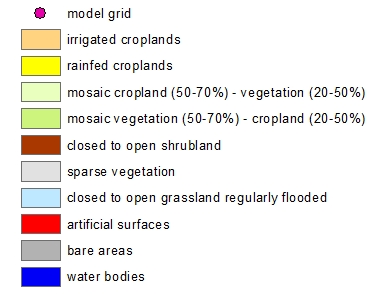
\includegraphics{../tex/extracted-media/media/image12.wmf}

where E\textsubscript{λ} is the solar spectral irradiance expressed in W / (m\textsuperscript{2}·nanometre) at wavelength λ and dλ is the wave-\\
length interval used in the summation. S\textsubscript{er} λ is the erythema reference action spectrum, and k\textsubscript{er} is a constant\\
equal to 40 m\textsuperscript{2} / W.

\textbf{Product discipline 0 -- Meteorological products, parameter category 5: long-wave radiation}

Number Parameter Units

0 Net long-wave radiation flux (surface)* W m\textsuperscript{--2}

1 Net long-wave radiation flux (top of atmosphere)* W m\textsuperscript{--2}

2 Long-wave radiation flux* W m\textsuperscript{--2}

3 Downward long-wave radiation flux W m\textsuperscript{--2}

4 Upward long-wave radiation flux W m\textsuperscript{--2}

5 Net long-wave radiation flux W m\textsuperscript{--2}

6 Net long-wave radiation flux, clear sky W m\textsuperscript{--2}

7 Brightness temperature K

8 Downward long-wave radiation flux, clear sky W m\textsuperscript{--2}

9--191 Reserved

192--254 Reserved for local use

255 Missing

\textbf{\_\_\_\_\_\_\_\_\_\_\_\_\_\_\_\_\_\_\_\_\_\_}

* Parameter deprecated. See Regulation 92.6.2 and use another parameter instead.

\textbf{Product discipline 0 -- Meteorological products, parameter category 6: cloud}

Number Parameter Units

0 Cloud ice kg m\textsuperscript{--2}

1 Total cloud cover \%

2 Convective cloud cover \%

3 Low cloud cover \%

4 Medium cloud cover \%

5 High cloud cover \%

6 Cloud water kg m\textsuperscript{--2}

7 Cloud amount \%

8 Cloud type (Code table 4.203)

9 Thunderstorm maximum tops m

10 Thunderstorm coverage (Code table 4.204)

11 Cloud base m

12 Cloud top m

13 Ceiling m

14 Non-convective cloud cover \%

15 Cloud work function J kg\textsuperscript{--1}

16 Convective cloud efficiency Proportion

17 Total condensate* kg kg\textsuperscript{--1}

18 Total column-integrated cloud water* kg m\textsuperscript{--2}

\emph{(continued)}

\emph{\\
(Code table 4.2 -- continued)}

Number Parameter Units

19 Total column-integrated cloud ice* kg m\textsuperscript{--2}

20 Total column-integrated condensate* kg m\textsuperscript{--2}

21 Ice fraction of total condensate Proportion

22 Cloud cover \%

23 Cloud ice mixing ratio* kg kg\textsuperscript{--1}

24 Sunshine Numeric

25 Horizontal extent of cumulonimbus (CB) \%

26 Height of convective cloud base m

27 Height of convective cloud top m

28 Number of cloud droplets per unit mass of air kg\textsuperscript{--1}

29 Number of cloud ice particles per unit mass of air kg\textsuperscript{--1}

30 Number density of cloud droplets m\textsuperscript{--3}

31 Number density of cloud ice particles m\textsuperscript{--3}

32 Fraction of cloud cover Numeric

33 Sunshine duration s

34 Surface long-wave effective total cloudiness Numeric

35 Surface short-wave effective total cloudiness Numeric

36 Fraction of stratiform precipitation cover Proportion

37 Fraction of convective precipitation cover Proportion

38 Mass density of cloud droplets kg m\textsuperscript{--3}

39 Mass density of cloud ice kg m\textsuperscript{--3}

40 Mass density of convective cloud water droplets kg m\textsuperscript{--3}

41--46 Reserved

47 Volume fraction of cloud water droplets** Numeric

48 Volume fraction of cloud ice particles** Numeric

49 Volume fraction of cloud (ice and/or water)** Numeric

50--191 Reserved

192--254 Reserved for local use

255 Missing

\_\_\_\_\_\_\_\_\_\_\_\_\_\_\_\_\_\_\_\_\_

* Parameter deprecated. Use another parameter in parameter category 1: moisture instead.

** The sum of the water and ice fractions may exceed the total due to overlap between the volumes containing\\
ice and those containing liquid water.

\textbf{Product discipline 0 -- Meteorological products, parameter category 7: thermodynamic stability\\
indices}

Number Parameter Units

0 Parcel lifted index (to 500 hPa) K

1 Best lifted index (to 500 hPa) K

2 K index K

3 KO index K

4 Total totals index K

5 Sweat index Numeric

6 Convective available potential energy J kg\textsuperscript{--1}

\emph{(continued)}

\emph{\\
(Code table 4.2 -- continued)}

Number Parameter Units

7 Convective inhibition J kg\textsuperscript{--1}

8 Storm relative helicity J kg\textsuperscript{--1}

9 Energy helicity index Numeric

10 Surface lifted index K

11 Best (4-layer) lifted index K

12 Richardson number Numeric

13 Showalter index K

14 Reserved

15 Updraught helicity m\textsuperscript{2} s\textsuperscript{--2}

16 Bulk Richardson number Numeric

17 Gradient Richardson number Numeric

18 Flux Richardson number Numeric

19 Convective available potential energy -- shear m\textsuperscript{2} s\textsuperscript{--2}

20--191 Reserved

192--254 Reserved for local use

255 Missing

\textbf{Product discipline 0 -- Meteorological products, parameter category 13: aerosols}

Number Parameter Units

0 Aerosol type (Code table 4.205)

1--191 Reserved

192--254 Reserved for local use

255 Missing

\textbf{Product discipline 0 -- Meteorological products, parameter category 14: trace gases}

Number Parameter Units

0 Total ozone DU

1 Ozone mixing ratio kg kg\textsuperscript{--1}

2 Total column integrated ozone DU

3--191 Reserved

192--254 Reserved for local use

255 Missing

\textbf{Product discipline 0 -- Meteorological products, parameter category 15: radar}

Number Parameter Units

0 Base spectrum width m s\textsuperscript{--1}

1 Base reflectivity dB

2 Base radial velocity m s\textsuperscript{--1}

3 Vertically integrated liquid water (VIL) kg m\textsuperscript{--2}

4 Layer-maximum base reflectivity dB

5 Precipitation kg m\textsuperscript{--2}

6 Radar spectra (1) --

7 Radar spectra (2) --

8 Radar spectra (3) --

9 Reflectivity of cloud droplets dB

\emph{(continued)}

\emph{\\
(Code table 4.2 -- continued)}

Number Parameter Units

10 Reflectivity of cloud ice dB

11 Reflectivity of snow dB

12 Reflectivity of rain dB

13 Reflectivity of graupel dB

14 Reflectivity of hail dB

15 Hybrid scan reflectivity dB

16 Hybrid scan reflectivity height m

17--191 Reserved

192--254 Reserved for local use

255 Missing

\textbf{Product Discipline 0 -- Meteorological products, parameter category 16: forecast radar imagery}

Number Parameter Units

0 Equivalent radar reflectivity factor for rain mm\textsuperscript{6} m\textsuperscript{--3}

1 Equivalent radar reflectivity factor for snow mm\textsuperscript{6} m\textsuperscript{--3}

2 Equivalent radar reflectivity factor for mm\textsuperscript{6} m\textsuperscript{--3}\\
parameterized convection

3 Echo top m

4 Reflectivity dB

5 Composite reflectivity dB

6--191 Reserved

192--254 Reserved for local use

255 Missing

Note: Decibel (dB) is a logarithmic measure of the relative power, or of the relative values of two flux densities, especially of sound intensities and radio and radar power densities. In radar meteorology, the logarithmic scale (dBZ) is used for measuring radar reflectivity factor (obtained from the American Meteorological Society \emph{Glossary of Meteorology}).

\textbf{Product discipline 0 -- Meteorological products, parameter category 17: electrodynamics}

Number Parameter Units

0 Lightning strike density m\textsuperscript{--2} s\textsuperscript{--1}

1 Lightning potential index (LPI) (see Note) J kg\textsuperscript{--1}

2 Cloud-to-ground lightning flash density km\textsuperscript{--2} day\textsuperscript{--1}

3 Cloud-to-cloud lightning flash density km\textsuperscript{--2} day\textsuperscript{--1}

4 Total Lightning flash density (see Note 2) km\textsuperscript{--2} day\textsuperscript{--1}

Notes:

(1) Definition of LPI after Lynn et al.: Lynn, B. and Y. Yair, 2010: Prediction of lightning flash density with the WRF model, \emph{Adv. Geosci}., 23:11--16; Yair, Y., B. Lynn, C. Price, V. Kotroni, K. Lagouvardos, E. Morin, A. Mugnai and M. Llasat, 2010: Predicting the potential for lightning activity in Mediterranean storms based on the Weather Research and Forecasting (WRF) model dynamic and microphysical fields, \emph{Journal of Geophysical Research}, 115, D04205, doi:10.1029/2008JD010868.

(2) The total lightning flash density is the sum of cloud-to-ground and cloud-to-cloud lightning flash densities (see Lopez, P., 2016: A lightning parameterization for the ECMWF Integrated Forecasting System, \emph{Monthly Weather Review}, 144, 3057--3075).

\emph{(continued)}

\emph{\\
(Code table 4.2 -- continued)}

\textbf{Product discipline 0 -- Meteorological products, parameter category 18: nuclear/radiology}

Number Parameter Units

0 Air concentration of caesium 137 Bq m\textsuperscript{--3}

1 Air concentration of iodine 131 Bq m\textsuperscript{--3}

2 Air concentration of radioactive pollutant Bq m\textsuperscript{--3}

3 Ground deposition of caesium 137 Bq m\textsuperscript{--2}

4 Ground deposition of iodine 131 Bq m\textsuperscript{--2}

5 Ground deposition of radioactive pollutant Bq m\textsuperscript{--2}

6 Time-integrated air concentration of caesium Bq s m\textsuperscript{--3}\\
pollutant (see Note 1)

7 Time-integrated air concentration of iodine Bq s m\textsuperscript{--3}\\
pollutant (see Note 1)

8 Time-integrated air concentration of radioactive Bq s m\textsuperscript{--3}\\
pollutant (see Note 1)

9 Reserved

10 Air concentration (see Note 2) Bq m\textsuperscript{--3}

11 Wet deposition Bq m\textsuperscript{\emph{--}2}

12 Dry deposition Bq m\textsuperscript{\emph{--}2}

13 Total deposition (wet + dry) Bq m\textsuperscript{\emph{--}2}

14 Specific activity concentration (see Note 2) Bq kg\textsuperscript{--1}

15 Maximum of air concentration in layer Bq m\textsuperscript{--3}

16 Height of maximum air concentration m

17 Column-integrated air concentration Bq m\textsuperscript{--2}

18 Column-averaged air concentration in layer Bq m\textsuperscript{--3}

19--191 Reserved

192--254 Reserved for local use

255 Missing

Notes:

(1) Statistical process 1 (Accumulation) does not change units. It is recommended to use another parameter without the word ``time-integrated'' in its name and accumulation in PDT.

(2) Conversion factor between ``Specific activity concentration'' (14) and ``Air concentration'' (10) is ``mass density''\\
{[}kg m\textsuperscript{--3}{]}.

(3) Parameters from 10 onward may be used in combination with product definition templates 4.40-- 4.43 and Common Code table C--14 (Code table 4.230) to represent any type of radioisotope.

\textbf{Product discipline 0 -- Meteorological products, parameter category 19: physical atmospheric properties}

Number Parameter Units

0 Visibility m

1 Albedo \%

2 Thunderstorm probability \%

3 Mixed layer depth m

4 Volcanic ash (Code table 4.206)

5 Icing top m

6 Icing base m

7 Icing (Code table 4.207)

8 Turbulence top m

9 Turbulence base m

10 Turbulence (Code table 4.208)

11 Turbulent kinetic energy J kg\textsuperscript{--1}

\emph{(continued)}

\emph{\\
(Code table 4.2 -- continued)}

Number Parameter Units

12 Planetary boundary-layer regime (Code table 4.209)

13 Contrail intensity (Code table 4.210)

14 Contrail engine type (Code table 4.211)

15 Contrail top m

16 Contrail base m

17 Maximum snow albedo (see Note 1) \%

18 Snow free albedo \%

19 Snow albedo \%

20 Icing \%

21 In-cloud turbulence \%

22 Clear air turbulence (CAT) \%

23 Supercooled large droplet probability (see Note 2) \%

24 Convective turbulent kinetic energy J kg\textsuperscript{--1}

25 Weather (Code table 4.225)

26 Convective outlook (Code table 4.224)

27 Icing scenario (Code table 4.227)

28 Mountain wave turbulence (eddy dissipation rate) m\textsuperscript{2/3} s\textsuperscript{--1}

29 Clear air turbulence (CAT) m\textsuperscript{2/3} s\textsuperscript{--1}

30 Eddy dissipation parameter (see Note 3) m\textsuperscript{2/3} s\textsuperscript{--1}

31 Maximum of eddy dissipation parameter in layer m\textsuperscript{2/3} s\textsuperscript{--1}

32 Highest freezing level m

33 Visibility through liquid fog m

34 Visibility through ice fog m

35 Visibility through blowing snow m

36--191 Reserved

192--254 Reserved for local use

255 Missing

Notes:

(1) Parameter deprecated. See Regulation 92.6.2 and use another parameter instead.

(2) Supercooled large droplets (SLD) are defined as those with a diameter greater than 50 microns.

(3) Eddy dissipation parameter is the third root of eddy dissipation rate {[}m\textsuperscript{2} s\textsuperscript{--3}{]}.

\textbf{Product discipline 0 -- Meteorological products, parameter category 20: atmospheric chemical\\
constituents}

Number Parameter Units

0 Mass density (concentration) kg m\textsuperscript{--3}

1 Column-integrated mass density (see Note 1) kg m\textsuperscript{--2}

2 Mass mixing ratio (mass fraction in air) kg kg\textsuperscript{--1}

3 Atmosphere emission mass flux kg m\textsuperscript{--2} s\textsuperscript{--1}

4 Atmosphere net production mass flux kg m\textsuperscript{--2} s\textsuperscript{--1}

5 Atmosphere net production and emission mass flux kg m\textsuperscript{--2} s\textsuperscript{--1}

6 Surface dry deposition mass flux kg m\textsuperscript{--2} s\textsuperscript{--1}

7 Surface wet deposition mass flux kg m\textsuperscript{--2} s\textsuperscript{--1}

8 Atmosphere re-emission mass flux kg m\textsuperscript{--2} s\textsuperscript{--1}

\emph{(continued)}

\emph{\\
(Code table 4.2 -- continued)}

Number Parameter Units

9 Wet deposition by large-scale precipitation mass kg m\textsuperscript{--2} s\textsuperscript{--1}\\
flux

10 Wet deposition by convective precipitation mass kg m\textsuperscript{--2} s\textsuperscript{--1}\\
flux

11 Sedimentation mass flux kg m\textsuperscript{--2} s\textsuperscript{--1}

12 Dry deposition mass flux kg m\textsuperscript{--2} s\textsuperscript{--1}

13 Transfer from hydrophobic to hydrophilic kg kg\textsuperscript{--1} s\textsuperscript{--1}

14 Transfer from SO\textsubscript{2} (sulphur dioxide) to SO\textsubscript{4} kg kg\textsuperscript{--1} s\textsuperscript{--1}\\
(sulphate)

15--49 Reserved

50 Amount in atmosphere mol

51 Concentration in air mol m\textsuperscript{--3}

52 Volume mixing ratio (fraction in air) mol mol\textsuperscript{--1}

53 Chemical gross production rate of concentration mol m\textsuperscript{--3} s\textsuperscript{--1}

54 Chemical gross destruction rate of concentration mol m\textsuperscript{--3} s\textsuperscript{--1}

55 Surface flux mol m\textsuperscript{--2} s\textsuperscript{--1}

56 Changes of amount in atmosphere (see Note 1) mol s\textsuperscript{--1}

57 Total yearly average burden of the atmosphere mol

58 Total yearly averaged atmospheric loss mol s\textsuperscript{--1}\\
(see Note 1)

59 Aerosol number concentration (see Note 2) m\textsuperscript{--3}

60 Aerosol specific number concentration kg\textsuperscript{--1}\\
(see Note 2)

61 Maximum of mass density in layer (see Note 1) kg m\textsuperscript{--3}

62 Height of maximum mass density m

63 Column-averaged mass density in layer kg m\textsuperscript{--3}

64--99 Reserved

100 Surface area density (aerosol) m\textsuperscript{--1}

101 Vertical visual range m

102 Aerosol optical thickness Numeric

103 Single scattering albedo Numeric

104 Asymmetry factor Numeric

105 Aerosol extinction coefficient m\textsuperscript{--1}

106 Aerosol absorption coefficient m\textsuperscript{--1}

107 Aerosol lidar backscatter from satellite m\textsuperscript{--1} sr\textsuperscript{--1}

108 Aerosol lidar backscatter from the ground m\textsuperscript{--1} sr\textsuperscript{--1}

109 Aerosol lidar extinction from satellite m\textsuperscript{--1}

110 Aerosol lidar extinction from the ground m\textsuperscript{--1}

111 Angstrom exponent Numeric

112--191 Reserved

192--254 Reserved for local use

255 Missing

Notes:

(1) FirstFixedSurface and SecondFixedSurface of Code table 4.5 (Fixed surface types and units) to define the vertical extent, i.e. FirstFixedSurface can be set to 1 (Ground or water surface) and SecondFixedSurface set to 7 (Tropopause) for a restriction to the troposphere.

\emph{(continued)}\textbf{\\
}

\emph{(Code table 4.2 -- continued)}

(2) The term ``number density'' is used as well for ``number concentration'' (code number 59); conversion factor between ``number density'' (59) and ``specific number concentration'' (60) is ``mass density'' {[}kg m\textsuperscript{--3}{]}.

\textbf{Product discipline 0 -- Meteorological products, parameter category 190: CCITT IA5 string}

Number Parameter Units

0 Arbitrary text string CCITT IA5

1--191 Reserved

192--254 Reserved for local use

255 Missing

\textbf{Product discipline 0 -- Meteorological products, parameter category 191: miscellaneous}

Number Parameter Units

0 Seconds prior to initial reference time s\\
(defined in Section 1)

1 Geographical latitude °N

2 Geographical longitude °E

3 Days since last observation d

4--191 Reserved

192--254 Reserved for local use

255 Missing

\textbf{Product discipline 1 -- Hydrological products, parameter category 0: hydrology basic products}

Number Parameter Units

0 Flash flood guidance kg m\textsuperscript{--2}\\
(Encoded as an accumulation over a floating\\
subinterval of time between the reference time\\
and valid time)

1 Flash flood runoff kg m\textsuperscript{--2}\\
(Encoded as an accumulation over a floating\\
subinterval of time)

2 Remotely sensed snow cover (Code table 4.215)

3 Elevation of snow-covered terrain (Code table 4.216)

4 Snow water equivalent per cent of normal \%

5 Baseflow-groundwater runoff kg m\textsuperscript{--2}

6 Storm surface runoff kg m\textsuperscript{--2}

7 Discharge from rivers or streams m\textsuperscript{3} s\textsuperscript{--1}

8 Groundwater upper storage kg m\textsuperscript{--2}

9 Groundwater lower storage kg m\textsuperscript{--2}

10 Side flow into river channel m\textsuperscript{3} s\textsuperscript{--1} m\textsuperscript{--1}

11 River storage of water m\textsuperscript{3}

12 Floodplain storage of water m\textsuperscript{3}

13 Depth of water on soil surface kg m\textsuperscript{--2}

14 Upstream accumulated precipitation kg m\textsuperscript{--2}

15 Upstream accumulated snow melt kg m\textsuperscript{--2}

16 Percolation rate kg m\textsuperscript{--2} s\textsuperscript{--1}

17--191 Reserved

\emph{(continued)}

\emph{\\
(Code table 4.2 -- continued)}

Number Parameter Units

192--254 Reserved for local use

255 Missing

Notes:

(1) Remotely sensed snow cover is expressed as a field of dimensionless, thematic values. The currently accepted values are for no-snow/no-cloud, 50, for clouds, 100, and for snow, 250 (see Code table 4.215).

(2) A data field representing snow coverage by elevation portrays at which elevations there is a snow pack. The elevation values typically range from 0 to 90 in 100-metre increments. A value of 253 is used to represent a no-snow/no-cloud data point. A value of 254 is used to represent a data point at which snow elevation could not be estimated because of clouds obscuring the remote sensor (when using aircraft or satellite measurements).

(3) Snow water equivalent per cent of normal is stored in per cent of normal units. For example, a value of 110 indicates 110 per cent of the normal snow water equivalent for a given depth of snow.

\textbf{Product discipline 1 -- Hydrological products, parameter category 1: hydrology probabilities}

Number Parameter Units

0 Conditional per cent precipitation amount kg m\textsuperscript{--2}\\
fractile for an overall period\\
(Encoded as an accumulation)

1 Per cent precipitation in a sub-period of an \%\\
overall period\\
(Encoded as per cent accumulation over\\
the sub-period)

2 Probability of 0.01 inch of precipitation (POP) \%

3--191 Reserved

192--254 Reserved for local use

255 Missing

\textbf{Product discipline 1 -- Hydrological products, parameter category 2: inland water and\\
sediment properties}

Number Parameter Units

0 Water depth m

1 Water temperature K

2 Water fraction Proportion

3 Sediment thickness m

4 Sediment temperature K

5 Ice thickness m

6 Ice temperature K

7 Ice cover Proportion

8 Land cover (0 = water, 1 = land) Proportion

9 Shape factor with respect to salinity profile --

10 Shape factor with respect to temperature --\\
profile in thermocline

11 Attenuation coefficient of water with respect m\textsuperscript{--1}\\
to solar radiation

12 Salinity kg kg\textsuperscript{--1}

13 Cross-sectional area of flow in channel m\textsuperscript{2}

\emph{(continued)}

\emph{\\
(Code table 4.2 -- continued)}

\textbf{Product discipline 2 -- Land surface products, parameter category 0: vegetation/biomass}

Number Parameter Units

0 Land cover (0 = sea, 1 = land) Proportion

1 Surface roughness m

2 Soil temperature*** K

3 Soil moisture content* kg m\textsuperscript{--2}

4 Vegetation \%

5 Water runoff kg m\textsuperscript{--2}

6 Evapotranspiration kg\textsuperscript{--2} s\textsuperscript{--1}

7 Model terrain height m

8 Land use (Code table 4.212)

9 Volumetric soil moisture content** Proportion

10 Ground heat flux* W m\textsuperscript{--2}

11 Moisture availability \%

12 Exchange coefficient kg m\textsuperscript{--2} s\textsuperscript{--1}

13 Plant canopy surface water kg m\textsuperscript{--2}

14 Blackadar's mixing length scale m

15 Canopy conductance m s\textsuperscript{--1}

16 Minimal stomatal resistance s m\textsuperscript{--1}

17 Wilting point* Proportion

18 Solar parameter in canopy conductance Proportion

19 Temperature parameter in canopy Proportion

20 Humidity parameter in canopy conductance Proportion

21 Soil moisture parameter in canopy conductance Proportion

22 Soil moisture*** kg m\textsuperscript{--3}

23 Column-integrated soil water*** kg m\textsuperscript{--2}

24 Heat flux W m\textsuperscript{--2}

25 Volumetric soil moisture m\textsuperscript{3} m\textsuperscript{--3}

26 Wilting point kg m\textsuperscript{--3}

27 Volumetric wilting point m\textsuperscript{3} m\textsuperscript{--3}

28 Leaf area index Numeric

29 Evergreen forest cover Proportion

30 Deciduous forest cover Proportion

31 Normalized differential vegetation index (NDVI) Numeric

32 Root depth of vegetation m

33 Water runoff and drainage**** kg m\textsuperscript{--2}

34 Surface water runoff**** kg m\textsuperscript{--2}

35 Tile class Code table 4.243

36 Tile fraction Proportion

37 Tile percentage \%

38 Soil volumetric ice content (water equivalent) m\textsuperscript{3} m\textsuperscript{--3}\\
(see Note)

39--191 Reserved

192--254 Reserved for local use

255 Missing

\emph{(continued)}

\emph{\\
}

\emph{(Code table 4.2 -- continued)}

Note: For parameter 38 (Parameter category 0), ice volume is expressed as if the ice content were melted to liquid water and then its volume measured in the liquid state. This may be understood in the same manner as water equivalent snow depth.

\_\_\_\_\_\_\_\_\_\_\_\_\_\_\_\_\_\_\_\_\_

* Parameter deprecated. See Regulation 92.6.2 and use another parameter instead.

** It is recommended not to use this parameter, but another one with a more descriptive unit.

*** Parameter deprecated. Use another parameter in parameter category 3: soil products instead.

**** Statistical process 1 (Accumulation) does not change units.

\textbf{Product discipline 2 -- Land surface products, parameter category 3: soil products}

Number Parameter Units

0 Soil type (Code table 4.213)

1 Upper layer soil temperature* K

2 Upper layer soil moisture* kg m\textsuperscript{--3}

3 Lower layer soil moisture* kg m\textsuperscript{--3}

4 Bottom layer soil temperature* K

5 Liquid volumetric soil moisture (non-frozen)** Proportion

6 Number of soil layers in root zone Numeric

7 Transpiration stress-onset (soil moisture)** Proportion

8 Direct evaporation cease (soil moisture)** Proportion

9 Soil porosity** Proportion

10 Liquid volumetric soil moisture (non-frozen) m\textsuperscript{3} m\textsuperscript{--3}

11 Volumetric transpiration stress-onset (soil moisture) m\textsuperscript{3} m\textsuperscript{--3}

12 Transpiration stress-onset (soil moisture) kg m\textsuperscript{--3}

13 Volumetric direct evaporation cease (soil moisture) m\textsuperscript{3} m\textsuperscript{--3}

14 Direct evaporation cease (soil moisture) kg m\textsuperscript{--3}

15 Soil porosity m\textsuperscript{3} m\textsuperscript{--3}

16 Volumetric saturation of soil moisture m\textsuperscript{3} m\textsuperscript{--3}

17 Saturation of soil moisture kg m\textsuperscript{--3}

18 Soil temperature K

19 Soil moisture kg m\textsuperscript{--3}

20 Column-integrated soil moisture kg m\textsuperscript{--2}

21 Soil ice kg m\textsuperscript{--3}

22 Column-integrated soil ice kg m\textsuperscript{--2}

23 Liquid water in snow pack kg m\textsuperscript{--2}

24 Frost index K day\textsuperscript{--1}

25 Snow depth at elevation bands kg m\textsuperscript{--2}

26 Soil heat flux W m\textsuperscript{--2}

27 Soil depth m

28--191 Reserved

192--254 Reserved for local use

255 Missing

\_\_\_\_\_\_\_\_\_\_\_\_\_\_\_\_\_\_\_\_\_\_

* Parameter deprecated. See Regulation 92.6.2 and use another parameter instead.

** It is recommended not to use this parameter, but another one with a more descriptive unit.

\emph{(continued)}

\emph{\\
(Code table 4.2 -- continued)}

\textbf{Product discipline 2 -- Land surface products, parameter category 4: fire weather products}

Number Parameter Units

0 Fire outlook Code table 4.224

1 Fire outlook due to dry thunderstorm Code table 4.224

2 Haines index Numeric

3 Fire burned area \%

4 Fosberg index* Numeric

5 Forest Fire Weather Index (Canadian Forest Numeric\\
Service)

6 Fine Fuel Moisture Code (Canadian Forest Numeric\\
Service)

7 Duff Moisture Code (Canadian Forest Service) Numeric

8 Drought Code (Canadian Forest Service) Numeric

9 Initial Fire Spread Index (Canadian Forest Service) Numeric

10 Fire Buildup Index (Canadian Forest Service) Numeric

11 Fire Daily Severity Rating (Canadian Forest Service) Numeric

12--191 Reserved

192--254 Reserved for local use

255 Missing

\_\_\_\_\_\_\_\_\_\_\_\_\_\_\_\_\_\_\_\_\_\_

* The Fosberg index denotes the potential influence of weather on a wildland fire. It takes into account the combined effects of temperature, wind speed, relative humidity and precipitation. Higher values indicate a higher potential impact.

\textbf{Product discipline 2 -- Land surface products, parameter category 5: glaciers and inland ice}

Number Parameter Units

1 Glacier temperature K

\textbf{Product discipline 3 -- Space products, parameter category 0: image format products}

Number Parameter Units

0 Scaled radiance Numeric

1 Scaled albedo Numeric

2 Scaled brightness temperature Numeric

3 Scaled precipitable water Numeric

4 Scaled lifted index Numeric

5 Scaled cloud top pressure Numeric

6 Scaled skin temperature Numeric

7 Cloud mask Code table 4.217

8 Pixel scene type Code table 4.218

9 Fire detection indicator Code table 4.223

10--191 Reserved

192--254 Reserved for local use

255 Missing

\emph{(continued)}

\emph{\\
(Code table 4.2 -- continued)}

\textbf{Product discipline 3 -- Space products, parameter category 1: quantitative products}

Number Parameter Units

0 Estimated precipitation kg m\textsuperscript{--2}

1 Instantaneous rain rate kg m\textsuperscript{--2} s\textsuperscript{--1}

2 Cloud top height m

3 Cloud top height quality indicator Code table 4.219

4 Estimated u-component of wind m s\textsuperscript{--1}

5 Estimated v-component of wind m s\textsuperscript{--1}

6 Number of pixel used Numeric

7 Solar zenith angle °

8 Relative azimuth angle °

9 Reflectance in 0.6 micron channel \%

10 Reflectance in 0.8 micron channel \%

11 Reflectance in 1.6 micron channel \%

12 Reflectance in 3.9 micron channel \%

13 Atmospheric divergence s\textsuperscript{--1}

14 Cloudy brightness temperature K

15 Clear-sky brightness temperature K

16 Cloudy radiance (with respect to wave number) W m\textsuperscript{--1} sr\textsuperscript{--1}

17 Clear-sky radiance (with respect to wave W m\textsuperscript{--1} sr\textsuperscript{--1}\\
number)

18 Reserved

19 Wind speed m s\textsuperscript{--1}

20 Aerosol optical thickness at 0.635 μm

21 Aerosol optical thickness at 0.810 μm

22 Aerosol optical thickness at 1.640 μm

23 Angstrom coefficient

24--26 Reserved

27 Bidirectional reflectance factor (see Note 1) numeric

28 Brightness temperature K

29 Scaled radiance (see Note 2) numeric

30--97 Reserved

98 Correlation coefficient between MPE rain rates Numeric\\
for the co-located IR data and the microwave\\
data rain rates

99 Standard deviation between MPE rain rates kg m\textsuperscript{--2} s\textsuperscript{--1}\\
for the co-located IR data and the microwave\\
data rain rates

100--191 Reserved

192--254 Reserved for local use

255 Missing

Notes:

(1) The ratio of the radiant flux reflected by a surface to that reflected into the same reflected-beam geometry and wavelength range by an ideal (lossless) and diffuse (Lambertian) standard surface, irradiated under the same conditions.

(2) Top of atmosphere radiance observed by a sensor, multiplied by pi and divided by the in-band solar irradiance.

\emph{(continued)}

\emph{\\
(Code table 4.2 -- continued)}

\textbf{Product discipline 3 -- Space products, parameter category 2: cloud properties}

Number Parameter Units

0 Clear sky probability \%

1 Cloud top temperature K

2 Cloud top pressure Pa

3 Cloud type Code table 4.218

4 Cloud phase Code table 4.218

5 Cloud optical depth Numeric

6 Cloud particle effective radius m

7 Cloud liquid water path kg m\textsuperscript{--2}

8 Cloud ice water path kg m\textsuperscript{--2}

9 Cloud albedo Numeric

10 Cloud emissivity Numeric

11 Effective absorption optical depth ratio Numeric

30 Measurement cost Numeric

31 Upper layer cloud optical depth Numeric

32 Upper layer cloud top pressure Pa

33 Upper layer cloud effective radius m

34 Error in upper layer cloud optical depth Numeric

35 Error in upper layer cloud top pressure Pa

36 Error in upper layer cloud effective radius m

37 Lower layer cloud optical depth Numeric

38 Lower layer cloud top pressure Pa

39 Error in lower layer cloud optical depth Numeric

40 Error in lower layer cloud top pressure Pa

Note: Numbers 31 to 40 are deprecated.

\textbf{Product discipline 3 -- Space products, parameter category 3: flight rule conditions}

Number Parameter Units

0 Probability of encountering marginal visual flight \%\\
rule conditions

1 Probability of encountering low instrument flight \%\\
rule conditions

2 Probability of encountering instrument flight \%\\
rule conditions

\textbf{Product discipline 3 -- Space products, parameter category 4: volcanic ash}

Number Parameter Units

0 Volcanic ash probability \%

1 Volcanic ash cloud top temperature K

2 Volcanic ash cloud top pressure Pa

3 Volcanic ash cloud top height m

4 Volcanic ash cloud emissivity Numeric

5 Volcanic ash effective absorption optical depth Numeric\\
ratio

6 Volcanic ash cloud optical depth Numeric

7 Volcanic ash column density kg m\textsuperscript{--2}

8 Volcanic ash particle effective radius m

\emph{(continued)}

\emph{\\
(Code table 4.2 -- continued)}

\textbf{Product discipline 3 -- Space products, parameter category 5: sea-surface temperature}

Number Parameter Units

0 Interface sea-surface temperature (see Note 1) K

1 Skin sea-surface temperature (see Note 2) K

2 Sub-skin sea-surface temperature (see Note 3) K

3 Foundation sea-surface temperature (see Note 4) K

4 Estimated bias between sea-surface K\\
temperature and standard

5 Estimated standard deviation between sea- K\\
surface temperature and standard

Notes:

(1) Theoretical temperature at the precise air-sea interface.

(2) Temperature of the water across a very small depth (approximately the upper 20 micrometers).

(3) Temperature at the base of the thermal skin layer.

(4) Temperature of the water column free of diurnal temperature variability or equal to the SST sub-skin in the absence of any diurnal signal.

\textbf{Product discipline 3 -- Space products, parameter category 6: solar radiation}

Number Parameter Units

0 Global solar irradiance (see Note 1) W m\textsuperscript{--2}

1 Global solar exposure (see Note 2) J m\textsuperscript{--2}

2 Direct solar irradiance (see Note 3) W m\textsuperscript{--2}

3 Direct solar exposure (see Note 4) J m\textsuperscript{--2}

4 Diffuse solar irradiance (see Note 5) W m\textsuperscript{--2}

5 Diffuse solar exposure (see Note 6) J m\textsuperscript{--2}

Notes:

(1) The solar flux per unit area received from a solid angle of 2π sr on a horizontal surface.

(2) Time integral of global solar irradiance.

(3) The solar flux per unit area received from the solid angle of the sun's disc on a surface normal to the sun direction.

(4) Time integral of direct solar irradiance.

(5) The solar flux per unit area received from a solid angle of 2π sr, except for the solid angle of the sun's disc, on a horizontal surface.

(6) Time integral of diffuse solar irradiance.

\textbf{Product discipline 10 -- Oceanographic products, parameter category 0: waves}

Number Parameter Units

0 Wave spectra (1) --

1 Wave spectra (2) --

2 Wave spectra (3) --

3 Significant height of combined wind waves m\\
and swell

4 Direction of wind waves degree true

5 Significant height of wind waves m

6 Mean period of wind waves s

7 Direction of swell waves degree true

8 Significant height of swell waves m

\emph{(continued)}

\emph{\\
(Code table 4.2 -- continued)}

Number Parameter Units

9 Mean period of swell waves s

10 Primary wave direction degree true

11 Primary wave mean period s

12 Secondary wave direction degree true

13 Secondary wave mean period s

14 Direction of combined wind waves and swell degree true

15 Mean period of combined wind waves and swell s

16 Coefficient of drag with waves --

17 Friction velocity m s\textsuperscript{--1}

18 Wave stress N m\textsuperscript{--2}

19 Normalized wave stress --

20 Mean square slope of waves --

21 u-component surface Stokes drift m s\textsuperscript{--1}

22 v-component surface Stokes drift m s\textsuperscript{--1}

23 Period of maximum individual wave height s

24 Maximum individual wave height m

25 Inverse mean wave frequency s

26 Inverse mean frequency of wind waves s

27 Inverse mean frequency of total swell s

28 Mean zero-crossing wave period s

29 Mean zero-crossing period of wind waves s

30 Mean zero-crossing period of total swell s

31 Wave directional width --

32 Directional width of wind waves --

33 Directional width of total swell --

34 Peak wave period s

35 Peak period of wind waves s

36 Peak period of total swell s

37 Altimeter wave height m

38 Altimeter corrected wave height m

39 Altimeter range relative correction --

40 10-metre neutral wind speed over waves m s--1

41 10-metre wind direction over waves °

42 Wave energy spectrum m\textsuperscript{2} s rad\textsuperscript{--1}

43 Kurtosis of the sea-surface elevation due to --\\
waves

44 Benjamin--Feir index --

45 Spectral peakedness factor s\textsuperscript{--1}

46 Peak wave direction °

47 Significant wave height of first swell partition m

48 Significant wave height of second swell partition m

49 Significant wave height of third swell partition m

50 Mean wave period of first swell partition s

51 Mean wave period of second swell partition s

52 Mean wave period of third swell partition s

53 Mean wave direction of first swell partition °

\emph{(continued)}

\emph{\\
(Code table 4.2 -- continued)}

Number Parameter Units

54 Mean wave direction of second swell partition °

55 Mean wave direction of third swell partition °

56--191 Reserved

192--254 Reserved for local use

255 Missing

* Further information concerning the wave parameters can be found in the \emph{Guide to Wave Analysis and Forecasting} (WMO-No. 702).

\textbf{Product discipline 10 -- Oceanographic products, parameter category 1: currents}

Number Parameter Units

0 Current direction degree true

1 Current speed m s\textsuperscript{--1}

2 u-component of current m s\textsuperscript{--1}

3 v-component of current m s\textsuperscript{--1}

4 \textbf{Rip current occurrence probability \%}

5--191 Reserved

192--254 Reserved for local use

255 Missing

\textbf{Product discipline 10 -- Oceanographic products, parameter category 2: ice}

Number Parameter Units

0 Ice cover Proportion

1 Ice thickness m

2 Direction of ice drift degree true

3 Speed of ice drift m s\textsuperscript{--1}

4 u-component of ice drift m s\textsuperscript{--1}

5 v-component of ice drift m s\textsuperscript{--1}

6 Ice growth rate m s\textsuperscript{--1}

7 Ice divergence s\textsuperscript{--1}

8 Ice temperature K

9 Module of ice internal pressure* Pa m

10 Zonal vector component of vertically Pa m\\
integrated ice internal pressure

11 Meridional vector component of vertically Pa m\\
integrated ice internal pressure

12 Compressive ice strength N m\textsuperscript{--1}

13--191 Reserved

192--254 Reserved for local use

255 Missing

* Ice internal pressure or stress (Pa m) is the integrated pressure across the vertical thickness of a layer of ice. It is produced when concentrated ice reacts to external forces such as wind and ocean currents.

\emph{(continued)}

\emph{\\
(Code table 4.2 -- continued)}

\textbf{Product discipline 10 -- Oceanographic products, parameter category 3: surface properties}

Number Parameter Units

0 Water temperature K

1 Deviation of sea level from mean m

2 Heat exchange coefficient --

3--191 Reserved

192--254 Reserved for local use

255 Missing

\textbf{Product discipline 10 -- Oceanographic products, parameter category 4: subsurface properties}

Number Parameter Units

0 Main thermocline depth m

1 Main thermocline anomaly m

2 Transient thermocline depth m

3 Salinity kg kg\textsuperscript{--1}

4 Ocean vertical heat diffusivity m\textsuperscript{2} s\textsuperscript{--1}

5 Ocean vertical salt diffusivity m\textsuperscript{2} s\textsuperscript{--1}

6 Ocean vertical momentum diffusivity m\textsuperscript{2} s\textsuperscript{--1}

7 Bathymetry m

8--10 Reserved

11 Shape factor with respect to salinity profile --

12 Shape factor with respect to temperature --\\
profile in thermocline

13 Attenuation coefficient of water with respect to m\textsuperscript{--1}\\
solar radiation

14 Water depth m

15 Water temperature K

16--191 Reserved

192--254 Reserved for local use

255 Missing

\textbf{Product discipline 10 -- Oceanographic products, parameter category 191: miscellaneous}

Number Parameter Units

0 Seconds prior to initial reference time s\\
(defined in Section 1)

1 Meridional overturning stream function m\textsuperscript{3} s\textsuperscript{--1}

2 Reserved

3 Days since last observation d

4--191 Reserved

192--254 Reserved for local use

255 Missing

\emph{\textbf{\\
}}

\emph{\textbf{Code table 4.3}} \textbf{--} \emph{Type of generating process}

Code figure Meaning

0 Analysis

1 Initialization

2 Forecast

3 Bias corrected forecast

4 Ensemble forecast

5 Probability forecast

6 Forecast error

7 Analysis error

8 Observation

9 Climatological

10 Probability-weighted forecast

11 Bias-corrected ensemble forecast

12 Post-processed analysis (see Note)

13 Post-processed forecast (see Note)

14 Nowcast

15 Hindcast

16 Physical retrieval

17 Regression analysis

18 Difference between two forecasts

19--191 Reserved

192--254 Reserved for local use

255 Missing

Note: Code figures 12 and 13 are intended in cases where code figures 0 and 2 may not be sufficient to indicate that significant post-processing has taken place on an initial analysis or forecast output.

\textbf{Code table 4.4 -- \emph{Indicator of unit of time range}}

Code figure Meaning

0 Minute

1 Hour

2 Day

3 Month

4 Year

5 Decade (10 years)

6 Normal (30 years)

7 Century (100 years)

8--9 Reserved

10 3 hours

11 6 hours

12 12 hours

13 Second

14--191 Reserved

192--254 Reserved for local use

255 Missing

\textbf{\\
}

\textbf{Code table 4.5 -- \emph{Fixed surface types and units}}

Code figure Meaning Unit

0 Reserved

1 Ground or water surface --

2 Cloud base level --

3 Level of cloud tops --

4 Level of 0 °C isotherm --

5 Level of adiabatic condensation lifted from the surface --

6 Maximum wind level --

7 Tropopause --

8 Nominal top of the atmosphere --

9 Sea bottom --

10 Entire atmosphere --

11 Cumulonimbus (CB) base m

12 Cumulonimbus (CB) top m

13 Lowest level where vertically integrated cloud cover \%\\
exceeds the specified percentage (cloud base for a\\
given percentage cloud cover)

14 Level of free convection (LFC) --

15 Convective condensation level (CCL) --

16 Level of neutral buoyancy or equilibrium level (LNB) --

17--19 Reserved

20 Isothermal level K

21 Lowest level where mass density exceeds the specified kg m\textsuperscript{--3}\\
value (base for a given threshold of mass density)

22 Highest level where mass density exceeds the specified kg m\textsuperscript{--3}\\
value (top for a given threshold of mass density)

23 Lowest level where air concentration exceeds the specified Bq m\textsuperscript{--3}\\
value (base for a given threshold of air concentration)

24 Highest level where air concentration exceeds the specified Bq m\textsuperscript{--3}\\
value (top for a given threshold of air concentration)

25 Highest level where radar reflectivity exceeds dBZ

the specified value (echo top for a given threshold of\\
reflectivity)

26--99 Reserved

100 Isobaric surface Pa

101 Mean sea level

102 Specific altitude above mean sea level m

103 Specified height level above ground m

104 Sigma level ``sigma'' value

105 Hybrid level --

106 Depth below land surface m

107 Isentropic (theta) level K

108 Level at specified pressure difference from ground to level Pa

109 Potential vorticity surface K m\textsuperscript{2} kg\textsuperscript{--1} s\textsuperscript{--1}

110 Reserved

111 Eta level --

112 Reserved

113 Logarithmic hybrid level

114 Snow level Numeric

\emph{(continued)}

\emph{\\
(Code table 4.5 -- continued)}

Number Parameter Units

115 Sigma height level (see Note 4) --

116 Reserved

117 Mixed layer depth m

118 Hybrid height level --

119 Hybrid pressure level --

120--149 Reserved

150 Generalized vertical height coordinate (see Note 5) --

151 Soil level (see Note 6) Numeric

152--159 Reserved

160 Depth below sea level m

161 Depth below water surface m

162 Lake or river bottom --

163 Bottom of sediment layer --

164 Bottom of thermally active sediment layer --

165 Bottom of sediment layer penetrated by thermal wave --

166 Mixing layer --

167 Bottom of root zone --

168--173 Reserved

174 Top surface of ice on sea, lake or river --

175 Top surface of ice, under snow cover, on sea, lake or river --

176 Bottom surface (underside) ice on sea, lake or river --

177 Deep soil (of indefinite depth) --

178 Reserved

179 Top surface of glacier ice and inland ice --

180 Deep inland or glacier ice (of indefinite depth) --

181 Grid tile land fraction as a model surface --

182 Grid tile water fraction as a model surface --

183 Grid tile ice fraction on sea, lake or river as a model surface --

184 Grid tile glacier ice and inland ice fraction as a model surface --

185--191 Reserved

192--254 Reserved for local use

255 Missing

Notes:

(1) The Eta vertical coordinate system involves normalizing the pressure at some point on a specific level by the mean sea-level pressure at that point.

(2) Hybrid height level (Code figure 118) can be defined as:\\
z(k) = A(k) + B(k) x orog\\
(k = 1,...,NLevels; orog = orography; z(k) = height in metres at level k)

(3) Hybrid pressure level, for which Code figure 119 shall be used instead of 105, can be defined as:\\
p(k) = A(k) + B(k) x sp\\
(k = 1,...,NLevels; sp = surface pressure; p(k) = pressure at level k)

(4) Sigma height level is the vertical model level of the height-based terrain-following coordinate (Gal-Chen and Somerville, 1975). The value of the level = (height of the level -- height of the terrain) / (height of the top level -- height of the terrain), which is ≥ 0 and ≤ 1.

\emph{(continued)}

\emph{\\
(Code table 4.5 -- continued)}

(5) The definition of a generalized vertical height coordinate implies the absence of coordinate values in Section 4 but the presence of an external 3D-GRIB message that specifies the height of every model grid point in metres (see Notes to Section 4 in the section above entitled Specification of Octet Contents), i.e., this GRIB message will contain the field with discipline = 0, category = 3, parameter = 6 (Geometric height).

(6) The soil level represents a model level for which the depth is not constant across the model domain. The depth in metres of the level is provided by another GRIB message with the parameter "soil depth" with discipline 2, category~3 and parameter number 27.

\textbf{Code table 4.6 -- \emph{Type of ensemble forecast}}

Code figure Meaning

0 Unperturbed high-resolution control forecast

1 Unperturbed low-resolution control forecast

2 Negatively perturbed forecast

3 Positively perturbed forecast

4 Multi-model forecast

5--191 Reserved

192--254 Reserved for local use

255 Missing

\textbf{Code table 4.7 -- \emph{Derived forecast}}

Code figure Meaning

0 Unweighted mean of all members

1 Weighted mean of all members

2 Standard deviation with respect to cluster mean

3 Standard deviation with respect to cluster mean, normalized

4 Spread of all members

5 Large anomaly index of all members (see Note 1)

6 Unweighted mean of the cluster members

7 Interquartile range (range between the 25th and 75th quantile)

8 Minimum of all ensemble members (see Note 2)

9 Maximum of all ensemble members (see Note 2)

10--191 Reserved

192--254 Reserved for local use

255 Missing

Notes:

(1) Large anomaly index is defined as \{(number of members whose anomaly is higher than 0.5 x SD) -- (number of members whose anomaly is lower than --0.5 x SD)\} / (number of members) at each grid point, where SD is defined as observed climatological standard deviation.

(2) It should be noted that the reference for "minimum of all ensemble members" and "maximum of all ensemble members" is the set of ensemble members and not a time interval and should not be confused with the maximum and minimum described by PDT 4.8.

\textbf{\\
}

\textbf{Code table 4.8 -- \emph{Clustering method}}

Code figure Meaning

0 Anomaly correlation

1 Root mean square

2--191 Reserved

192--254 Reserved for local use

255 Missing

\textbf{Code table 4.9 -- \emph{Probability type}}

Code figure Meaning

0 Probability of event below lower limit

1 Probability of event above upper limit

2 Probability of event between lower and upper limits (the range includes the lower limit\\
but not the upper limit)

3 Probability of event above lower limit

4 Probability of event below upper limit

5 Probability of event equal to lower limit

6 Probability of event in above normal category (see Notes 1 and 2)

7 Probability of event in near normal category (see Notes 1 and 2)

8 Probability of event in below normal category (see Notes 1 and 2)

9--191 Reserved

192--254 Reserved for local use

255 Missing

Notes:

(1) Above normal, near normal and below normal are defined as three equiprobable categories based on climatology at each point over the geographical area covered by the grid. The type and methodology of the reference climatology are unspecified and should be documented concurrently by the data producer.

(2) Product definition templates that use Code Table 4.9 may contain octets to store the values of lower and upper limits. When categorical probability is used (such as below, near and above normal), these octets shall be set to ``all ones'' (missing).

\textbf{Code table 4.10 -- \emph{Type of statistical processing}}

Code figure Meaning

0 Average

1 Accumulation (see Note 1)

2 Maximum

3 Minimum

4 Difference (value at the end of time range minus value at the beginning)

5 Root mean square

6 Standard deviation

7 Covariance (temporal variance) (see Note 2)

8 Difference (value at the start of time range minus value at the end)

9 Ratio (see Note 3)

10 Standardized anomaly

11 Summation

12--191 Reserved

\emph{(continued)}

\emph{\\
(Code table 4.10 -- continued)}

Code figure Meaning

192--254 Reserved for local use

255 Missing

Notes:

(1) The original data value (Y in the note 4 of Regulation 92.9.4) has units of Code table 4.2 multiplied by second, unless otherwise noted on Code table 4.2.

(2) The original data value has squared units of Code table 4.2.

(3) The original data value is non-dimensional number without units.

\textbf{Code table 4.11 -- \emph{Type of time intervals}}

Code figure Meaning

0 Reserved

1 Successive times processed have same forecast time, start time of forecast is\\
incremented

2 Successive times processed have same start time of forecast, forecast time is\\
incremented

3 Successive times processed have start time of forecast incremented and forecast time\\
decremented so that valid time remains constant

4 Successive times processed have start time of forecast decremented and forecast time\\
incremented so that valid time remains constant

5 Floating subinterval of time between forecast time and end of overall time interval*

6--191 Reserved

192--254 Reserved for local use

255 Missing

\_\_\_\_\_\_\_\_\_\_\_\_\_\_\_\_\_\_\_\_

* Code figure 5 applies to instances where a single time subinterval was used to calculate the statistically processed field. The exact starting and ending times of the subinterval are not given, but it is known that it is contained inclusively between the beginning time and the ending time of the overall interval.

\textbf{Code table 4.12 -- \emph{Operating mode}}

Code figure Meaning

0 Maintenance mode

1 Clear air

2 Precipitation

3--191 Reserved

192--254 Reserved for local use

255 Missing

\textbf{Code table 4.13 -- \emph{Quality control indicator}}

Code figure Meaning

0 No quality control applied

1 Quality control applied

2--191 Reserved

192--254 Reserved for local use

255 Missing

\textbf{Code table 4.14 -- \emph{Clutter filter indicator}}

Code figure Meaning

0 No clutter filter used

1 Clutter filter used

2--191 Reserved

192--254 Reserved for local use

255 Missing

\textbf{Code table 4.15 -- \emph{Type of spatial processing used to arrive at given data value from the source data}}

Code figure Meaning

0 Data is calculated directly from the source grid with no interpolation (see Note 1)

1 Bilinear interpolation using the 4 source grid grid-point values surrounding the nominal\\
grid-point

2 Bicubic interpolation using the 4 source grid grid-point values surrounding the nominal\\
grid-point

3 Using the value from the source grid grid-point which is nearest to the nominal grid-point

4 Budget interpolation using the 4 source grid grid-point values surrounding the nominal\\
grid-point (see Note 2)

5 Spectral interpolation using the 4 source grid grid-point values surrounding the nominal\\
grid-point

6 Neighbor-budget interpolation using the 4 source grid grid-point values surrounding the\\
nominal grid-point (see Note 3)

7--191 Reserved

192--254 Reserved for local use

255 Missing

Notes:

(1) This method assumes that each field really represents box averages/maxima/minima where each box extends halfway to its neighboring grid point in each direction to represent averages/maxima/minima of values from the source grid with no interpolation.

(2) Budget interpolation means a low-order interpolation method that quasi-conserves area averages. It would be appropriate for interpolating budget fields such as precipitation. This method assumes that the field really represents box averages/maxima/minima where each box extends halfway to its neighboring grid point in each direction. The method actually averages bilinearly interpolated values in a square array of points distributed within each output grid box.

(3) Performs a budget interpolation at the grid point nearest to the nominal grid point.

\textbf{Code table 4.16} \emph{-- Quality value associated with parameter}

Code figure Meaning

0 Confidence index (see Note 2)

1 Quality indicator (see Note 3 and Code table 4.244)

2 Correlation of product with used calibration product (see Note 4)

3 Standard deviation (see Note 5)

4 Random error (see Note 5)

5-191 Reserved

192-254 Reserved for local use

255 Missing

\emph{(continued)}

\emph{\\
(Code table 4.16 -- continued)}

Notes:

(1) When a non-missing value is used from this code table, the original data value is a quality value associated with the parameter defined by octets 10 and 11 of the product definition template.

(2) The original data value is a non-dimensional number from 0 to 1, where 0 indicates no confidence and 1 indicates maximal confidence.

(3) The original data value is defined by Code table 4.244

(4) The original data value is a non-dimensional number without units.

(5) The original data value is in the same units as the parameter defined by octets 10 and 11 of the product definition template.

\textbf{Code table 4.91 -- \emph{Type of Interval}}

Code figure Meaning

0 Smaller than first limit

1 Greater than second limit

2 Between first and second limit. The range includes the first limit but not the second limit

3 Greater than first limit

4 Smaller than second limit

5 Smaller or equal first limit

6 Greater or equal second limit

7 Between first and second. The range includes the first limit and the second limit

8 Greater or equal first limit

9 Smaller or equal second limit

10 Between first and second limit. The range includes the second limit but not the first limit

11 Equal to first limit

12--191 Reserved

192--254 Reserved for local use

255 Missing

\textbf{Code table 4.201 -- \emph{Precipitation type}}

Code figure Meaning

0 Reserved

1 Rain

2 Thunderstorm

3 Freezing rain

4 Mixed/ice

5 Snow

6 Wet snow

7 Mixture of rain and snow

8 Ice pellets

9 Graupel

10 Hail

11 Drizzle

12 Freezing drizzle

13--191 Reserved

192--254 Reserved for local use

255 Missing

\textbf{Code table 4.202 -- \emph{Precipitable water category}}

Code figure Meaning

0--191 Reserved

192--254 Reserved for local use

255 Missing

\textbf{Code table 4.203 -- \emph{Cloud type}}

Code figure Meaning

0 Clear

1 Cumulonimbus

2 Stratus

3 Stratocumulus

4 Cumulus

5 Altostratus

6 Nimbostratus

7 Altocumulus

8 Cirrostratus

9 Cirrocumulus

10 Cirrus

11 Cumulonimbus -- ground-based fog beneath the lowest layer

12 Stratus -- ground-based fog beneath the lowest layer

13 Stratocumulus -- ground-based fog beneath the lowest layer

14 Cumulus -- ground-based fog beneath the lowest layer

15 Altostratus -- ground-based fog beneath the lowest layer

16 Nimbostratus -- ground-based fog beneath the lowest layer

17 Altocumulus -- ground-based fog beneath the lowest layer

18 Cirrostratus -- ground-based fog beneath the lowest layer

19 Cirrocumulus -- ground-based fog beneath the lowest layer

20 Cirrus -- ground-based fog beneath the lowest layer

21--190 Reserved

191 Unknown

192--254 Reserved for local use

255 Missing

Note: Code figures 11--20 indicate all four layers were used and ground-based fog is beneath the lowest layer.

\textbf{Code table 4.204 -- \emph{Thunderstorm coverage}}

Code figure Meaning

0 None

1 Isolated (1--2\%)

2 Few (3--5\%)

3 Scattered (6--45\%)

4 Numerous (\textgreater{} 45\%)

5--191 Reserved

192--254 Reserved for local use

255 Missing

\textbf{Code table 4.205 -- \emph{Presence of aerosol}}

Code figure Meaning

0 Aerosol not present

1 Aerosol present

2--191 Reserved

192--254 Reserved for local use

255 Missing

\textbf{Code table 4.206 -- \emph{Volcanic ash}}

Code figure Meaning

0 Not present

1 Present

2--191 Reserved

192--254 Reserved for local use

255 Missing

\textbf{Code table 4.207 -- \emph{Icing}}

Code figure Meaning

0 None

1 Light

2 Moderate

3 Severe

4 Trace

5 Heavy

6--191 Reserved

192--254 Reserved for local use

255 Missing

\textbf{Code table 4.208 -- \emph{Turbulence}}

Code figure Meaning

0 None (smooth)

1 Light

2 Moderate

3 Severe

4 Extreme

5--191 Reserved

192--254 Reserved for local use

255 Missing

\textbf{\\
}

\textbf{Code table 4.209 -- \emph{Planetary boundary-layer regime}}

Code figure Meaning

0 Reserved

1 Stable

2 Mechanically driven turbulence

3 Forced convection

4 Free convection

5--191 Reserved

192--254 Reserved for local use

255 Missing

\textbf{Code table 4.210 -- \emph{Contrail intensity}}

Code figure Meaning

0 Contrail not present

1 Contrail present

2--191 Reserved

192--254 Reserved for local use

255 Missing

\textbf{Code table 4.211 -- \emph{Contrail engine type}}

Code figure Meaning

0 Low bypass

1 High bypass

2 Non-bypass

3--191 Reserved

192--254 Reserved for local use

255 Missing

\textbf{Code table 4.212 -- \emph{Land use}}

Code figure Meaning

0 Reserved

1 Urban land

2 Agriculture

3 Range land

4 Deciduous forest

5 Coniferous forest

6 Forest/wetland

7 Water

8 Wetlands

9 Desert

10 Tundra

11 Ice

12 Tropical forest

13 Savannah

14--191 Reserved

192--254 Reserved for local use

255 Missing

\textbf{Code table 4.213 -- \emph{Soil type}}

Code figure Meaning

0 Reserved

1 Sand

2 Loamy sand

3 Sandy loam

4 Silt loam

5 Organic (redefined)

6 Sandy clay loam

7 Silt clay loam

8 Clay loam

9 Sandy clay

10 Silty clay

11 Clay

12--191 Reserved

192--254 Reserved for local use

255 Missing

\textbf{Code table 4.215 -- \emph{Remotely sensed snow coverage}}

Code figure Meaning

0--49 Reserved

50 No-snow/no-cloud

51--99 Reserved

100 Clouds

101--249 Reserved

250 Snow

251--254 Reserved for local use

255 Missing

\textbf{Code table 4.216 -- \emph{Elevation of snow-covered terrain}}

Code figure Meaning

0--90 Elevation in increments of 100 m

91--253 Reserved

254 Clouds

255 Missing

\textbf{Code table 4.217 -- \emph{Cloud mask type}}

Code figure Meaning

0 Clear over water

1 Clear over land

2 Cloud

3 No data

4--191 Reserved

192--254 Reserved for local use

255 Missing

\textbf{Code table 4.218 -- \emph{Pixel scene type}}

Code figure Meaning

0 No scene identified

1 Green needle-leafed forest

2 Green broad-leafed forest

3 Deciduous needle-leafed forest

4 Deciduous broad-leafed forest

5 Deciduous mixed forest

6 Closed shrub-land

7 Open shrub-land

8 Woody savannah

9 Savannah

10 Grassland

11 Permanent wetland

12 Cropland

13 Urban

14 Vegetation/crops

15 Permanent snow/ice

16 Barren desert

17 Water bodies

18 Tundra

19 Warm liquid water cloud

20 Supercooled liquid water cloud

21 Mixed-phase cloud

22 Optically thin ice cloud

23 Optically thick ice cloud

24 Multilayered cloud

25--96 Reserved

97 Snow/ice on land

98 Snow/ice on water

99 Sun-glint

100 General cloud

101 Low cloud/fog/stratus

102 Low cloud/stratocumulus

103 Low cloud/unknown type

104 Medium cloud/nimbostratus

105 Medium cloud/altostratus

106 Medium cloud/unknown type

107 High cloud/cumulus

108 High cloud/cirrus

109 High cloud/unknown

110 Unknown cloud type

111 Single Layer Water Cloud

112 Single Layer Ice Cloud

113--191 Reserved

192--254 Reserved for local use

255 Missing

\textbf{Code table 4.219 -- \emph{Cloud top height quality indicator}}

Code figure Meaning

0 Nominal cloud top height quality

1 Fog in segment

2 Poor quality height estimation

3 Fog in segment and poor quality height estimation

4--191 Reserved

192--254 Reserved for local use

255 Missing

\textbf{Code table 4.220 -- \emph{Horizontal dimension processed}}

Code figure Meaning

0 Latitude

1 Longitude

2--191 Reserved

192--254 Reserved for local use

255 Missing

\textbf{Code table 4.221 -- \emph{Treatment of missing data}}

Code figure Meaning

0 Not included

1 Extrapolated

2--191 Reserved

192--254 Reserved for local use

255 Missing

\textbf{Code table 4.222 -- \emph{Categorical result}}

Code figure Meaning

0 No

1 Yes

2--191 Reserved

192--254 Reserved for local use

255 Missing

\textbf{Code table 4.223 -- \emph{Fire detection indicator}}

Code figure Meaning

0 No fire detected

1 Possible fire detected

2 Probable fire detected

3 Missing

\textbf{\\
}

\textbf{Code table 4.224 -- \emph{Categorical outlook}}

Code figure Meaning

0 No risk area

1 Reserved

2 General thunderstorm risk area

3 Reserved

4 Slight risk area

5 Reserved

6 Moderate risk area

7 Reserved

8 High risk area

9--10 Reserved

11 Dry thunderstorm (dry lightning) risk area

12--13 Reserved

14 Critical risk area

15--17 Reserved

18 Extremely critical risk area

19--254 Reserved

255 Missing

\textbf{Code table 4.225 -- \emph{Weather}}

(see FM 94 BUFR/FM 95 CREX Code table 0 20 003 -- Present weather)

\textbf{Code table 4.227 -- \emph{Icing scenario (weather/cloud classification)}}

Code figure Meaning

0 None

1 General

2 Convective

3 Stratiform

4 Freezing

5--191 Reserved

192--254 Reserved for local use

255 Missing value

\textbf{Code table 4.230 -- \emph{Atmospheric chemical constituent type}}

(See Common Code table C--14)

\textbf{Code table 4.233 -- \emph{Aerosol type}}

(See Common Code table C--14)

\textbf{\\
}

\textbf{Code table 4.234 \emph{-- Canopy cover fraction (to be used as partitioned parameter in product definition template 4.53 or 4.54)}}

Code figure Meaning

1 Crops, mixed farming

2 Short grass

3 Evergreen needleleaf trees

4 Deciduous needleleaf trees

5 Deciduous broadleaf trees

6 Evergreen broadleaf trees

7 Tall grass

8 Desert

9 Tundra

10 Irrigated crops

11 Semidesert

12 Ice caps and glaciers

13 Bogs and marshes

14 Inland water

15 Ocean

16 Evergreen shrubs

17 Deciduous shrubs

18 Mixed forest

19 Interrupted forest

20 Water and land mixtures

\textbf{Code table 4.236 \emph{-- Soil texture fraction (to be used as partitioned parameter in product definition template 4.53 or 4.54)}}

Code figure Meaning

1 Coarse

2 Medium

3 Medium-fine

4 Fine

5 Very-fine

6 Organic

7 Tropical-organic

\textbf{Code table 4.240 -- \emph{Type of distribution function}}

Code figure Meaning

0 No specific distribution function given

1 Delta functions with spatially variable concentration and fixed diameters \emph{D\textsubscript{l}} (\emph{p}1) in metre\\
(see Note 1)

2 Delta functions with spatially variable concentration and fixed masses \emph{M\textsubscript{l}} (\emph{p}1) in kg\\
(see Note 2)

3 Gaussian (normal) distribution with spatially variable concentration and fixed mean\\
diameter \emph{D\textsubscript{l}} (\emph{p}1) and variance σ (\emph{p}2) (see Note 3)

4 Gaussian (normal) distribution with spatially variable concentration, mean diameter and\\
variance (see Note 4)

\emph{(continued)}

\emph{\\
(Code table 4.240 -- continued)}

Code figure Meaning

5 Log-normal distribution with spatially variable number density, mean diameter and\\
variance (see Note 5)

6 Log-normal distribution with spatially variable number density, mean diameter and fixed\\
variance σ (\emph{p}1) (see Note 6)

7 Log-normal distribution with spatially variable number density and mass density and fixed\\
variance σ (\emph{p}1) and fixed particle density ρ (\emph{p}2) (see Note 7)

8 No distribution function. The encoded variable is derived from variables characterized by\\
type of distribution function of type No. 7 (see above) with fixed variance σ (\emph{p}1) and fixed\\
particle density \emph{p} (\emph{p}2)

9-49151 Reserved

49152--65534 Reserved for local use

65535 Missing value

Notes:

(1) Bin model or delta function with \emph{N} concentrations \emph{c\textsubscript{l}(r)} in class (or mode) \emph{l}.\\
Concentration--density function:

\begin{quote}
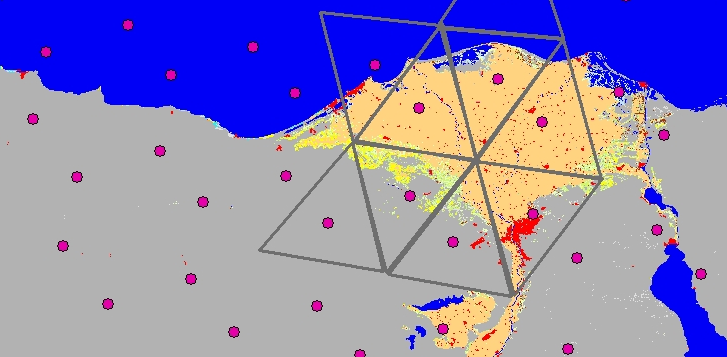
\includegraphics{../tex/extracted-media/media/image13.png}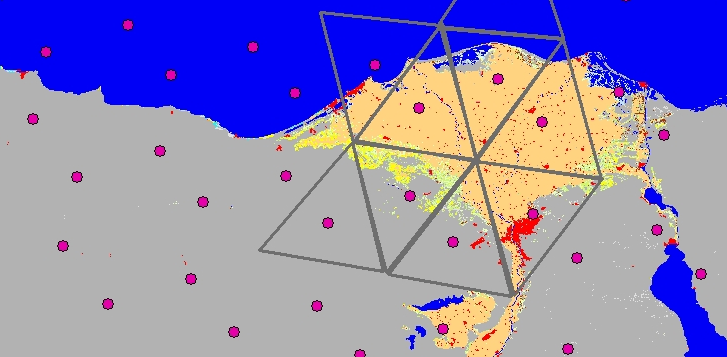
\includegraphics{../tex/extracted-media/media/image13.png}

where

\emph{N --} number of modes in the distribution

δ \emph{--} delta function

\emph{d --} diameter

\emph{D\textsubscript{l} --} diameter of mode \emph{l} (\emph{p}1)
\end{quote}

(2) Bin model or delta function with \emph{N} concentrations \emph{c\textsubscript{l}(r)} in class (or mode) \emph{l}.\\
Concentration--density function:

\begin{quote}
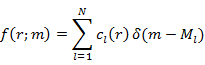
\includegraphics{../tex/extracted-media/media/image14.png}

where

\emph{N} -- number of modes in the distribution\\
δ \emph{--} delta function\\
\emph{m} \emph{--} mass\\
\emph{M\textsubscript{l }}-- mass of mode \emph{l} (\emph{p}1)
\end{quote}

(3) N-modal concentration--density function consisting of Gaussian functions:

\begin{quote}
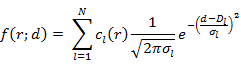
\includegraphics{../tex/extracted-media/media/image15.png}

where

\emph{N --} number of modes in the distribution\\
\emph{d --} diameter\\
\emph{D\textsubscript{l} --} mean diameter of mode \emph{l} (\emph{p}1)\\
σ\emph{\textsubscript{l} --} variance of mode \emph{l} (\emph{p}2)\\
with \emph{N} fields of concentration \emph{c\textsubscript{l}(r).}
\end{quote}

(4) N-modal concentration--density function consisting of Gaussian functions:

\begin{quote}
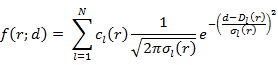
\includegraphics{../tex/extracted-media/media/image16.png}

with 3\emph{N} fields of concentration \emph{c\textsubscript{l}(r),} variance σ\emph{\textsubscript{l}(r)} and mean diameter \emph{D\textsubscript{l}(r).}
\end{quote}

\emph{(continued)}

\emph{\\
(Code table 4.240 -- continued)}

(5) N-modal log-normal-distribution for the number density:

\begin{quote}
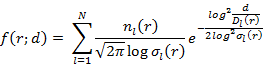
\includegraphics{../tex/extracted-media/media/image17.png}

where

\emph{d --} diameter\\
with 3\emph{N} fields of number density \emph{n\textsubscript{l}(r),} variance σ\emph{\textsubscript{l}(r)} and mean diameter \emph{D\textsubscript{l}(r).}
\end{quote}

(6) N-modal log-normal-distribution for the number density:

\begin{quote}
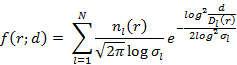
\includegraphics{../tex/extracted-media/media/image18.png}

where

σ\emph{\textsubscript{l} --} variance of mode \emph{l} (\emph{p}1)\\
with 2\emph{N} fields of number density \emph{n\textsubscript{l}(r)} and mean diameter \emph{D\textsubscript{l}(r)}.
\end{quote}

(7) N-modal log-normal-distribution for the number density as in Note 6, but with a prescribed mass density \emph{m\textsubscript{l}}(\emph{r}), from which the diameter \emph{D\textsubscript{l}(r)} is calculated by:

\begin{quote}
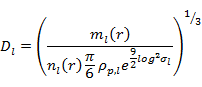
\includegraphics{../tex/extracted-media/media/image19.png}

where

σ\emph{\textsubscript{l} --} variance of mode \emph{l} (\emph{p}1)

ρ\textsubscript{p\emph{,}l} \emph{--} particle density (\emph{p}2)

with 2\emph{N} fields of number density \emph{n\textsubscript{l}(r)} and mass density \emph{m\textsubscript{l}(r).}
\end{quote}

\textbf{Code table 4.241 -- \emph{Coverage attributes}}

Code figure Meaning

0 Undefined

1 Unmodified

2 Snow covered

3 Flooded

4 Ice covered

5--191 Reserved

192--254 Reserved for local use

255 Missing value

\textbf{Code table 4.242 -- \emph{Tile classification}}

Code figure Meaning

0 Reserved

1 Land use classes according to ESA-GlobCover GCV2009

2 Land use classes according to European Commission--Global Land Cover Project GLC2000

3--191 Reserved

192--254 Reserved for local use

255 Missing value

\textbf{\\
}

\textbf{Code table 4.243 -- \emph{Tile class}}

Code figure Meaning

0 Reserved

1 Evergreen broadleaved forest

2 Deciduous broadleaved closed forest

3 Deciduous broadleaved open forest

4 Evergreen needle-leaf forest

5 Deciduous needle-leaf forest

6 Mixed leaf trees

7 Freshwater flooded trees

8 Saline water flooded trees

9 Mosaic tree/natural vegetation

10 Burnt tree cover

11 Evergreen shrubs closed-open

12 Deciduous shrubs closed-open

13 Herbaceous vegetation closed-open

14 Sparse herbaceous or grass

15 Flooded shrubs or herbaceous

16 Cultivated and managed areas

17 Mosaic crop/tree/natural vegetation

18 Mosaic crop/shrub/grass

19 Bare areas

20 Water

21 Snow and ice

22 Artificial surface

23 Ocean

24 Irrigated croplands

25 Rainfed croplands

26 Mosaic cropland (50--70\%) -- vegetation (20--50\%)

27 Mosaic vegetation (50--70\%) -- cropland (20--50\%)

28 Closed broadleaved evergreen forest

29 Closed needle-leaved evergreen forest

30 Open needle-leaved deciduous forest

31 Mixed broadleaved and needle-leaved forest

32 Mosaic shrubland (50--70\%) -- grassland (20--50\%)

33 Mosaic grassland (50--70\%) -- shrubland (20--50\%)

34 Closed to open shrubland

35 Sparse vegetation

36 Closed to open forest regularly flooded

37 Closed forest or shrubland permanently flooded

38 Closed to open grassland regularly flooded

39 Undefined

40--32767 Reserved

32768-- Reserved for local use

\textbf{\\
}

\textbf{Code table 4.244 -- \emph{Quality indicator}}

Code figure Meaning

0 No quality information available

1 Failed

2 Passed

3-191 Reserved

192-254 Reserved for local use

255 Missing

\_\_\_\_\_\_\_\_\_\_\_\_

\textbf{CODE TABLES USED IN SECTION 5}

\textbf{Code table 5.0 -- \emph{Data representation template number}}

Code figure Meaning

0 Grid point data -- simple packing

1 Matrix value at grid point -- simple packing

2 Grid point data -- complex packing

3 Grid point data -- complex packing and spatial differencing

4 Grid point data -- IEEE floating point data

5--39 Reserved

40 Grid point data -- JPEG 2000 code stream format

41 Grid point data -- Portable Network Graphics (PNG)

42 Grid point and spectral data -- CCSDS recommended lossless compression

43--49 Reserved

50 Spectral data -- simple packing

51 Spherical harmonics data -- complex packing

52--60 Reserved

61 Grid point data -- simple packing with logarithm pre-processing

62--199 Reserved

200 Run length packing with level values

201--49151 Reserved

49152--65534 Reserved for local use

65535 Missing

\textbf{Code table 5.1 -- \emph{Type of original field values}}

Code figure Meaning

0 Floating point

1 Integer

2--191 Reserved

192--254 Reserved for local use

255 Missing

\textbf{Code table 5.2 -- \emph{Matrix coordinate value function definition}}

Code figure Meaning

0 Explicit coordinate values set

1 Linear coordinates\\
f(1) = C1\\
f(n) = f(n--1) + C2

2--10 Reserved

11 Geometric coordinates\\
f(1) = C1\\
f(n) = C2 × f(n--1)

12--191 Reserved

192--254 Reserved for local use

255 Missing

\textbf{\\
}

\textbf{Code table 5.3 -- \emph{Matrix coordinate parameter}}

Code figure Meaning

1 Direction degrees true

2 Frequency (s\textsuperscript{--1})

3 Radial number (2pi/lambda) (m\textsuperscript{--1})

4--191 Reserved

192--254 Reserved for local use

255 Missing

\textbf{Code table 5.4 -- \emph{Group splitting method}}

Code figure Meaning

0 Row by row splitting

1 General group splitting

2--191 Reserved

192--254 Reserved for local use

255 Missing

\textbf{Code table 5.5 -- \emph{Missing value management for complex packing}}

Code figure Meaning

0 No explicit missing values included within data values

1 Primary missing values included within data values

2 Primary and secondary missing values included within data values

3--191 Reserved

192--254 Reserved for local use

255 Missing

\textbf{Code table 5.6 -- \emph{Order of spatial differencing}}

Code figure Meaning

0 Reserved

1 First-order spatial differencing

2 Second-order spatial differencing

3--191 Reserved

192--254 Reserved for local use

255 Missing

\textbf{Code table 5.7 -- \emph{Precision of floating-point numbers}}

Code figure Meaning

0 Reserved

1 IEEE 32-bit (I=4 in section 7)

2 IEEE 64-bit (I=8 in section 7)

3 IEEE 128-bit (I=16 in section 7)

4--254 Reserved

255 Missing

\textbf{\\
}

\textbf{Code table 5.40 -- \emph{Type of compression}}

Code figure Meaning

0 Lossless

1 Lossy

2--254 Reserved

255 Missing

\_\_\_\_\_\_\_\_\_\_\_\_\_\_\_

\textbf{CODE TABLES USED IN SECTION 6}

\textbf{Code table 6.0 -- \emph{Bit map indicator}}

Code figure Meaning

0 A bit map applies to this product and is specified in this Section

1--253 A bit map predetermined by the originating/generating centre applies to this product and is\\
not specified in this Section

254 A bit map defined previously in the same ``GRIB'' message applies to this product

255 A bit map does not apply to this product

\_\_\_\_\_\_\_\_\_\_\_\_\_\_\_
